%Version 3 December 2023
% See section 11 of the User Manual for version history
%
%%%%%%%%%%%%%%%%%%%%%%%%%%%%%%%%%%%%%%%%%%%%%%%%%%%%%%%%%%%%%%%%%%%%%%
%%                                                                 %%
%% Please do not use \input{...} to include other tex files.       %%
%% Submit your LaTeX manuscript as one .tex document.              %%
%%                                                                 %%
%% All additional figures and files should be attached             %%
%% separately and not embedded in the \TeX\ document itself.       %%
%%                                                                 %%
%%%%%%%%%%%%%%%%%%%%%%%%%%%%%%%%%%%%%%%%%%%%%%%%%%%%%%%%%%%%%%%%%%%%%

%%\documentclass[referee,sn-basic]{sn-jnl}% referee option is meant for double line spacing

%%=======================================================%%
%% to print line numbers in the margin use lineno option %%
%%=======================================================%%

%%\documentclass[lineno,sn-basic]{sn-jnl}% Basic Springer Nature Reference Style/Chemistry Reference Style

%%======================================================%%
%% to compile with pdflatex/xelatex use pdflatex option %%
%%======================================================%%

%%\documentclass[pdflatex,sn-basic]{sn-jnl}% Basic Springer Nature Reference Style/Chemistry Reference Style


%%Note: the following reference styles support Namedate and Numbered referencing. By default the style follows the most common style. To switch between the options you can add or remove “Numbered” in the optional parenthesis. 
%%The option is available for: sn-basic.bst, sn-vancouver.bst, sn-chicago.bst%  
 
%%\documentclass[pdflatex,sn-nature]{sn-jnl}% Style for submissions to Nature Portfolio journals
%%\documentclass[pdflatex,sn-basic]{sn-jnl}% Basic Springer Nature Reference Style/Chemistry Reference Style
%%\documentclass[pdflatex,sn-mathphys-num]{sn-jnl}% Math and Physical Sciences Numbered Reference Style 
%%\documentclass[pdflatex,sn-mathphys-ay]{sn-jnl}% Math and Physical Sciences Author Year Reference Style
%%\documentclass[pdflatex,sn-aps]{sn-jnl}% American Physical Society (APS) Reference Style
\documentclass[pdflatex,sn-vancouver,Numbered]{bst/sn-jnl}% Vancouver Reference Style
%%\documentclass[pdflatex,sn-apa]{sn-jnl}% APA Reference Style 
%%\documentclass[pdflatex,sn-chicago]{sn-jnl}% Chicago-based Humanities Reference Style


%%%% Standard Packages
%%<additional latex packages if required can be included here>

\usepackage{graphicx}%
\usepackage{multirow}%
\usepackage{amsmath,amssymb,amsfonts}%
\usepackage{amsthm}%
\usepackage{mathrsfs}%
\usepackage[title]{appendix}%
\usepackage{xcolor}%
\usepackage{textcomp}%
\usepackage{manyfoot}%
\usepackage{booktabs}%
\usepackage{algorithm}%
\usepackage{algorithmicx}%
\usepackage{algpseudocode}%
\usepackage{listings}%
\usepackage{booktabs}
\usepackage[graphicx]{realboxes}
\usepackage{graphicx}
\usepackage{adjustbox}
\usepackage{subcaption}
\usepackage{nameref}
\usepackage{verbatim}

%%%%

%%%%%=============================================================================%%%%
%%%%  Remarks: This template is provided to aid authors with the preparation
%%%%  of original research articles intended for submission to journals published 
%%%%  by Springer Nature. The guidance has been prepared in partnership with 
%%%%  production teams to conform to Springer Nature technical requirements. 
%%%%  Editorial and presentation requirements differ among journal portfolios and 
%%%%  research disciplines. You may find sections in this template are irrelevant 
%%%%  to your work and are empowered to omit any such section if allowed by the 
%%%%  journal you intend to submit to. The submission guidelines and policies 
%%%%  of the journal take precedence. A detailed User Manual is available in the 
%%%%  template package for technical guidance.
%%%%%=============================================================================%%%%

%% as per the requirement new theorem styles can be included as shown below
\theoremstyle{thmstyleone}%
\newtheorem{theorem}{Theorem}%  meant for continuous numbers
%%\newtheorem{theorem}{Theorem}[section]% meant for sectionwise numbers
%% optional argument [theorem] produces theorem numbering sequence instead of independent numbers for Proposition
\newtheorem{proposition}[theorem]{Proposition}% 
%%\newtheorem{proposition}{Proposition}% to get separate numbers for theorem and proposition etc.

\theoremstyle{thmstyletwo}%
\newtheorem{example}{Example}%
\newtheorem{remark}{Remark}%

\theoremstyle{thmstylethree}%
\newtheorem{definition}{Definition}%

\raggedbottom
%%\unnumbered% uncomment this for unnumbered level heads

% Macro: \dself{<mean>}{<std>}
\newcommand{\dself}[2]{$d_{\text{self}} = #1 \pm #2$}

% Macro: \dref{<mean>}{<std>}
\newcommand{\dref}[2]{$d_{\text{ref}} = #1 \pm #2$}

% Macro: \dselfdref{df}{tvalue}{pvalue}
% Exact p-value
\newcommand{\dselfdrefp}[3]{$d_{\text{self}} < d_{\text{ref}},\ \text{Welch's } t(#1) = #2,\ p = #3$}

% p-value as an upper bound
\newcommand{\dselfdrefpl}[3]{$d_{\text{self}} < d_{\text{ref}},\ \text{Welch's } t(#1) = #2,\ p < #3$}


\begin{document}

\title[Article Title]{Regularity of life rhythms}

%%=============================================================%%
%% GivenName	-> \fnm{Joergen W.}
%% Particle	-> \spfx{van der} -> surname prefix
%% FamilyName	-> \sur{Ploeg}
%% Suffix	-> \sfx{IV}
%% \author*[1,2]{\fnm{Joergen W.} \spfx{van der} \sur{Ploeg} 
%%  \sfx{IV}}\email{iauthor@gmail.com}
%%=============================================================%%

\author*[1]{\fnm{Nguyen} \sur{Luong}}\email{nguyen.luong@aalto.fi}


\author[1]{\fnm{Talayeh} \sur{Aledavood}}\email{talayeh.aledavood@aalto.fi}


\affil*[1]{\orgdiv{Computer Science}, \orgname{Aalto University} \city{Espoo}, \country{Finland}}

%%==================================%%
%% Sample for unstructured abstract %%
%%==================================%%

\abstract{Daily life is organised around recurrent activities to which people allocate their time. How person-specific are these routines? Using longitudinal behavioral data from four studies (n = XXX), we clustered daily activity features to derive an individual routine “signature” and quantified its persistence in two ways: the distribution of time across routine clusters and the transitions between clusters across adjacent segments. Across datasets, individuals maintain distinctive routine signatures that separate their life patterns from others. These signatures were stable over contiguous months but disappeared when observations were separated by long gaps. The findings imply that stable, person-specific routines can anchor personalised baselines and allow in-time interventions, should deviations from routines happen.}

\keywords{}

\maketitle


\section{Introduction}\label{sec1}
Humans’ daily lives are inherently synchronized with the 24-hour day–night cycle. This circadian rhythm shapes essential physiological and behavioural routines—such as sleep, physical activity, communication, and mobility. Maintaining the regularity of these routines are important for health, supporting well-being \cite{heintzelman2019routines}, enhancing life satisfaction \cite{margraf2016social}, and ensuring good sleep quality \cite{carney2006daily}. 

Human's daily routines are naturally stable, as individuals structure their activities to meet social, occupational, and environmental demands \cite{monk1994regularity}. This persistent property has been documented through structured surveys and diaries, which consistently reveal predictable temporal patterns (e.g., meal times, sleep schedules) and spatial regularities (e.g., commuting routes) \cite{hansonSystematicVariabilityRepetitious1988a, monk1990social, soehnerCircadianPreferenceSleepWake2011}. In modern times, the emerging ubiquity of personal digital devices has enabled large-scale, longitudinal analyses of human behaviour, confirming these findings with much higher resolution and longer observation period. For instance, studies using GPS and call-record data demonstrate that human's mobility follows highly predictable spatiotemporal trajectories, with individuals visiting a limited set of familiar locations in stable sequences \cite{songLimitsPredictabilityHuman2010, song2010modelling, alessandretti2020scales}. Similarly, individual's communication patterns display distinctive and persistent structures. Saramaki et al. conceptualized this structure as the social signature \cite{saramaki2014persistence}—the characteristic way individuals distribute communication effort across contacts. These signatures are found in different communication means (calls, SMS, emails) and remain robust despite substantial turnover in individual's social networks \cite{saramaki2014persistence, aledavoodDailyRhythmsMobile2015a, heydari2018multichannel, loriteLongTermEvolutionEmail2016}. Routine persistence also extends from the physical world to the digital domain, with high individual-level predictability observed in the timing and frequency of web visits \cite{barbosa2016returners, hu2018life, kulshrestha2021web} as well as in app usage patterns \cite{malmi2016you, kosinski2013private, petersSocialMediaUse2024}. Collectively, these findings suggest that persistence is not limited to a single behavioural modality, but rather reflects a general property of human behaviour observable across multiple domains and space.

Nonetheless, several gaps remain in understanding how individual routines persist. First, most prior work has focused on single behavioural domains, making it unclear whether persistence generalizes to multimodal routines - such as a combination of sleep, activity, mobility, and device usage. Multimodal data introduce additional complexity, as the interplay between different routines emerges. For example, late-night phone use often co-occurs with delayed bedtimes, while increased mobility may align with reduced device engagement. Second, while it is well known that ...

Latent-behaviour approaches offer a powerful way to address these challenges by assuming that daily life can be represented as a mixture of a limited set of recurring patterns. An early approach by Eagle et al. introduced the concept of eigenbehaviours \cite{eagleEigenbehaviorsIdentifyingStructure2009a}, showing that a small number of principal components could explain most variance in daily activity. This concept has been extended to different contexts, like quantifying latent mobility classes from GPS or mobility diaries \cite{jiangClusteringDailyPatterns2012, yangIdentifyingLatentActivity2023a}. Other decomposition methods—including non-negative matrix factorization \cite{aledavood2022quantifying, girardiniAdaptationStudentBehavioural2023a}, Latent Dirichlet Allocation \cite{farrahiDiscoveringRoutinesLargescale2011, farrahiWhatDidYou2008}, and Gaussian Mixture Models (GMM) \cite{zhou2022predicting, yan2025relapse}—have revealed hidden behavioural structures and linked their shifts to clinical or contextual outcomes. However, these studies have not systematically quantified how persistent such latent routines are, nor have they examined how persistence varies across populations and environments.

In this work, we introduce an approach for quantifying the persistence of multimodal daily routines. We model each individual’s daily behaviour as a mixture of Gaussian latent routine classes, capturing recurring patterns across domains such as sleep, activity, and device usage. Building on the concept of the social signature, we define the resulting distribution over these latent routines as a routine signature, representing how individuals allocate time across behavioural patterns. We further introduce the transition signature, which captures the stability of day-to-day transitions between routine types. We hypothesise that both signatures are highly individual-specific, remain stable over months, and can reliably distinguish individuals across time.

Using multimodal behavioural data from three distinct populations, we evaluate the persistence of these signatures and identify demographic and contextual factors underlying individual differences. Across datasets, we find that individuals exhibit stable and distinctive routine signatures, both in time allocation and in transitions between routines. These patterns are more similar within individuals than between individuals and remain robust across short (weeks) and long (months) observation windows. Crucially, we show that these properties generalize across diverse populations, suggesting that the structure and persistence of daily routines are universal features of human behaviour.

\section*{Results}\label{sec:results}  


\subsection*{Routine cluster characteristics}\label{sec:results:cluster}

Daily routines were quantified across three behavioral domains: device use, physical activity, and sleep. Behaviors were summarized by timing in four daily segments (morning, afternoon, evening, night) and by total daily duration (e.g., total screen time), yielding a 16-dimensional representation for each day (Methods). Using data from 1104 participants and over 153,000 person-days across three studies (S1–S3), we applied unsupervised clustering to each study to identify latent patterns of daily behavior (z-scored per participtants to focus on individual variability). For each study, the optimal cluster number was determined from model fit indices and the average Bhattycharya distance between clusters - higher distance suggest more separated clusters (see \nameref{sec:methods}). Model selection favored a full-covariance GMM with optimal component counts of 8, 11, and 8 for S1-S3. Given the marginal improvement for K=11 in S2, we proceeded with K=8 for all studies. Tuning details can be found in Supplementary.

\begin{figure}[htbp!]
    \centering
    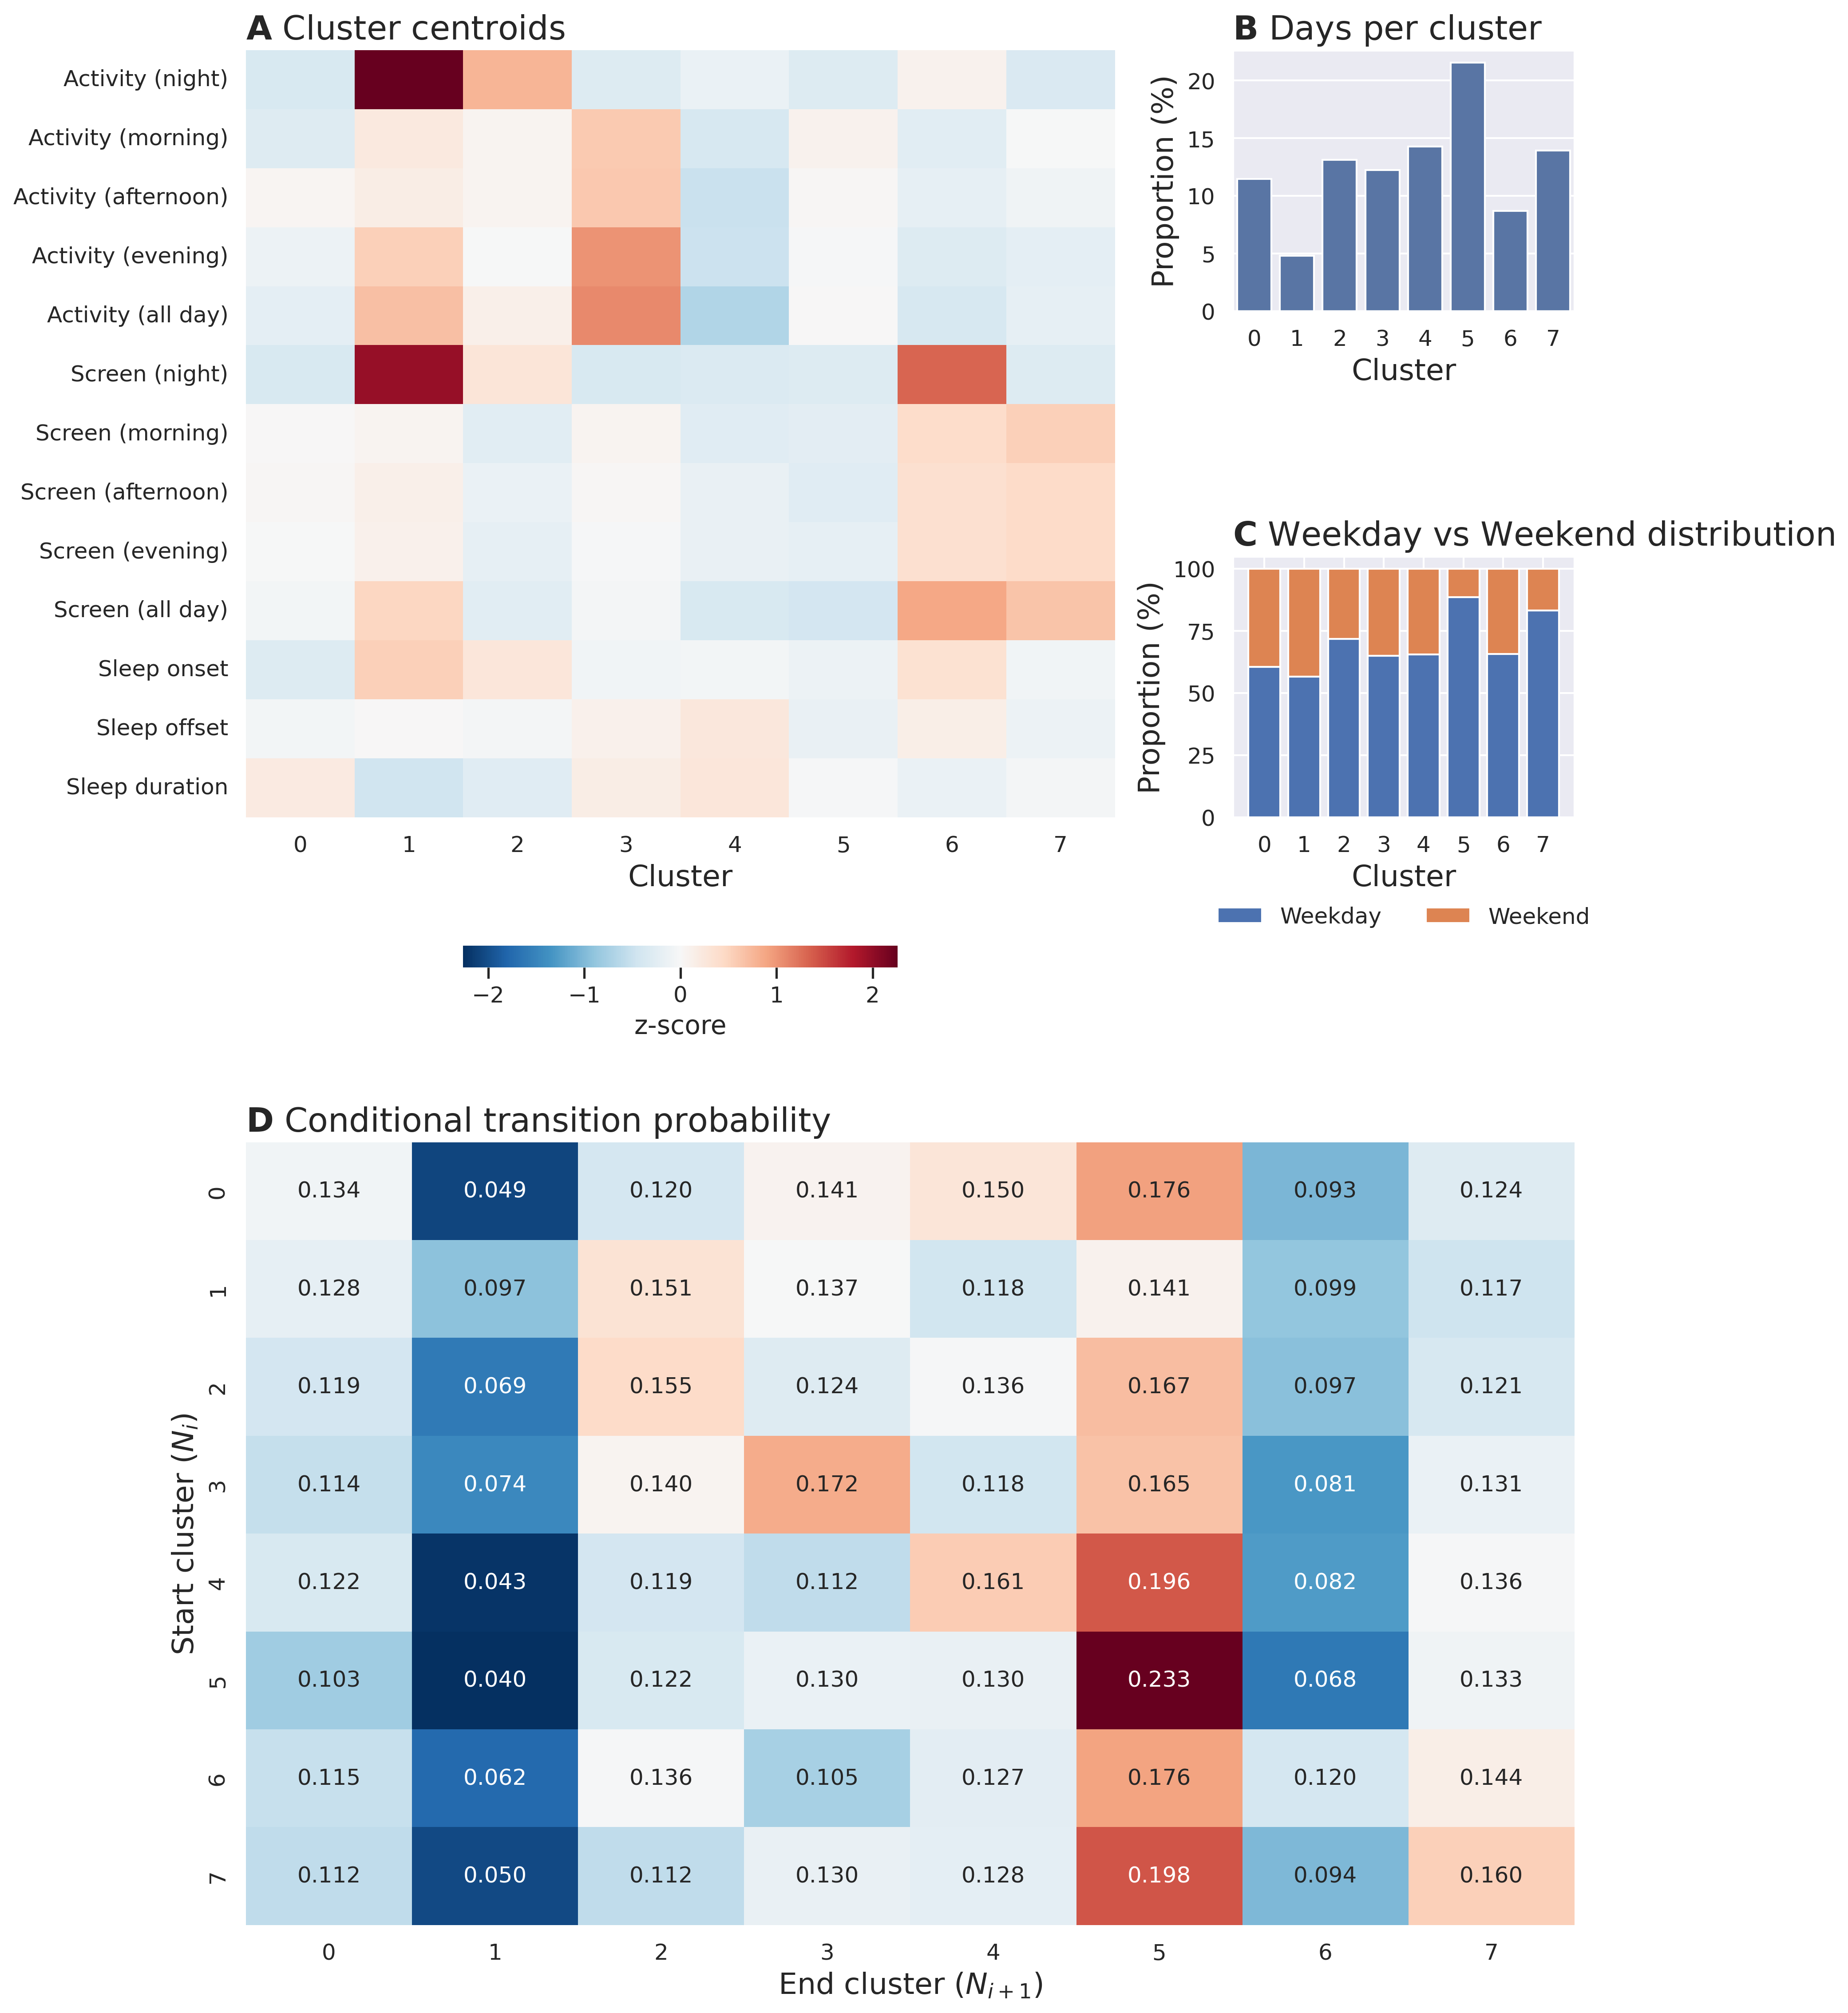
\includegraphics[width=1\linewidth]{figures/tesserae_summary.png}
    \caption{Cluster summary for S1. (A) Cluster centroids: Heatmap showing the average standardized feature values (z-scores) for each behavioral feature within each cluster. Each feature’s z-score is computed per individual to reflect within-person deviations. Higher (red) and lower (blue) values represent positive and negative deviations from an individual’s mean, respectively. (B) Days per cluster: Histogram showing the distribution of all recorded days across clusters, aggregated across the study population. (C) Weekday–weekend distribution: Stacked bar plot depicting the proportion of weekdays (blue) and weekends (orange) within each cluster. Certain clusters exhibit a significant weekend skew, depicting leisure-oriented behaviours that emerge on non-working days. (D) Heatmap of adjacency matrix depicting the conditional transition probability between cluster pairs. Transition probabilities are computed and normalized per participant, then averaged across participants to obtain a population means. Higher values indicate more frequent transitions.}
    \label{fig:tesserae-cluster-summary}
\end{figure}

In S1, a total of 592 participants and 106172 person-days were included in this analysis. The cluster profiles (centroids) are shown in \autoref{fig:tesserae-cluster-summary}A, with each cell showing the deviations from individual baseline.  One dominant cluster presenting the most typical routine (see \autoref{fig:tesserae-cluster-summary}B, characterized by all features sitting near the mean level and a small dip in screen usage. This cluster represents a typical workday of the white-collar cohort. As shown in \autoref{fig:tesserae-cluster-summary}C, some smaller clusters emerged, depicting different weekend patterns. They are characterized by increase in screen usage (Cluster x), increase nightly physical activity (Cluster x), or a increase in sleep duration. Organic weekend-weekday patterns naturally arise from the observations, given that temporal information was not provided during model fit. Clusters characteristics of S2 and S3 can be found in Supplementary xx.

To assess whether individuals tend to adhere to a single routine or frequently shift between different routine types, we analyzed the transition probabilities between clusters. For each participant, we constructed a transition matrix \(P\) by counting the number of transitions from cluster \(i\) to cluster \(j\), then normalizing each row so that the probabilities sum to 1 (see \nameref{sec:methods}). Each cell \(P_{ij}\) represents the probability of transitioning from routine \(i\) to routine \(j\), with larger values indicating more frequent transitions. If individuals were strongly adapted to a specific routine, we would expect the diagonal entries \(P_{ii}\) - denoting self-transitions - to have the highest values. However, this was not the case. As shown in \autoref{fig:tesserae-cluster-summary}D, most routine clusters converged toward a dominant cluster. The transition probabilities were also diffuse and asymmetric, indicating that the likelihood of moving between clusters varies across individuals. We repeated the analysis on S2 and S3 and observed similar results, suggesting that the asymmetry and diffuseness of routine transitions are consistent across different populations.

\begin{comment}
\begin{figure}[hbtp]
\centering
% Row 1
\begin{subfigure}{0.48\linewidth}
\centering
\includegraphics[width=\linewidth]{figures/globem_INS-W_1_summary.png}
\caption{INS--W 1}
\label{fig:globem:1}
\end{subfigure}\hfill
\begin{subfigure}{0.48\linewidth}
\centering
\includegraphics[width=\linewidth]{figures/globem_INS-W_2_summary.png}
\caption{INS--W 2}
\label{fig:globem:2}
\end{subfigure}

\medskip
% Row 2
\begin{subfigure}{0.48\linewidth}
\centering
\includegraphics[width=\linewidth]{figures/globem_INS-W_3_summary.png}
\caption{INS--W 3}
\label{fig:globem:3}
\end{subfigure}\hfill
\begin{subfigure}{0.48\linewidth}
\centering
\includegraphics[width=\linewidth]{figures/globem_INS-W_4_summary.png}
\caption{INS--W 4}
\label{fig:globem:4}
\end{subfigure}

\caption{GLOBEM summaries for INS--W splits (1--4).}
\label{fig:globem}
\end{figure}
\end{comment}

\subsection*{Persistence of individual's routine signature} \label{sec:results:signature_persistence}

For each participant and time segment, a \textit{routine signature} is defined as the vector of cluster proportions, sorted in descending order of frequency within that segment (\nameref{sec:methods}). To test whether an individual’s routine is more similar to their own than to others’, we compared the distributions of within-person distances \(d_{\text{self}}\) and between-person reference distances \(d_{\text{ref}}\) (see \autoref{fig:dself_dref}). For each participant \(i\), \(d_{\text{ref},i}\) was computed as the mean distance between \(i\)’s routine signature and those of all other participants, matched by time segment.

In S1 and S2, we retained participants with at least 270 days of data and divided them into three 90-day windows. In S3, we included participants who participated in at least two consecutive study waves. For S3, the reference distance \(d_{\text{ref}}\) was computed by comparing the routine signature of individual \(i\) between waves \(j\) and \(j+1\) against the signatures of all other participants in the same waves.

\autoref{fig:signature} shows the distribution of routine signatures across individuals and time segments. We find that, despite variability in total activity levels, individuals tend to allocate a large proportion of their time to a small number of routines, with the top three routines accounting for the majority of daily behaviour. This individuality is evident in the clear separation between participants’ signatures, even when observed months apart.

\begin{figure}[h!]
    \centering
    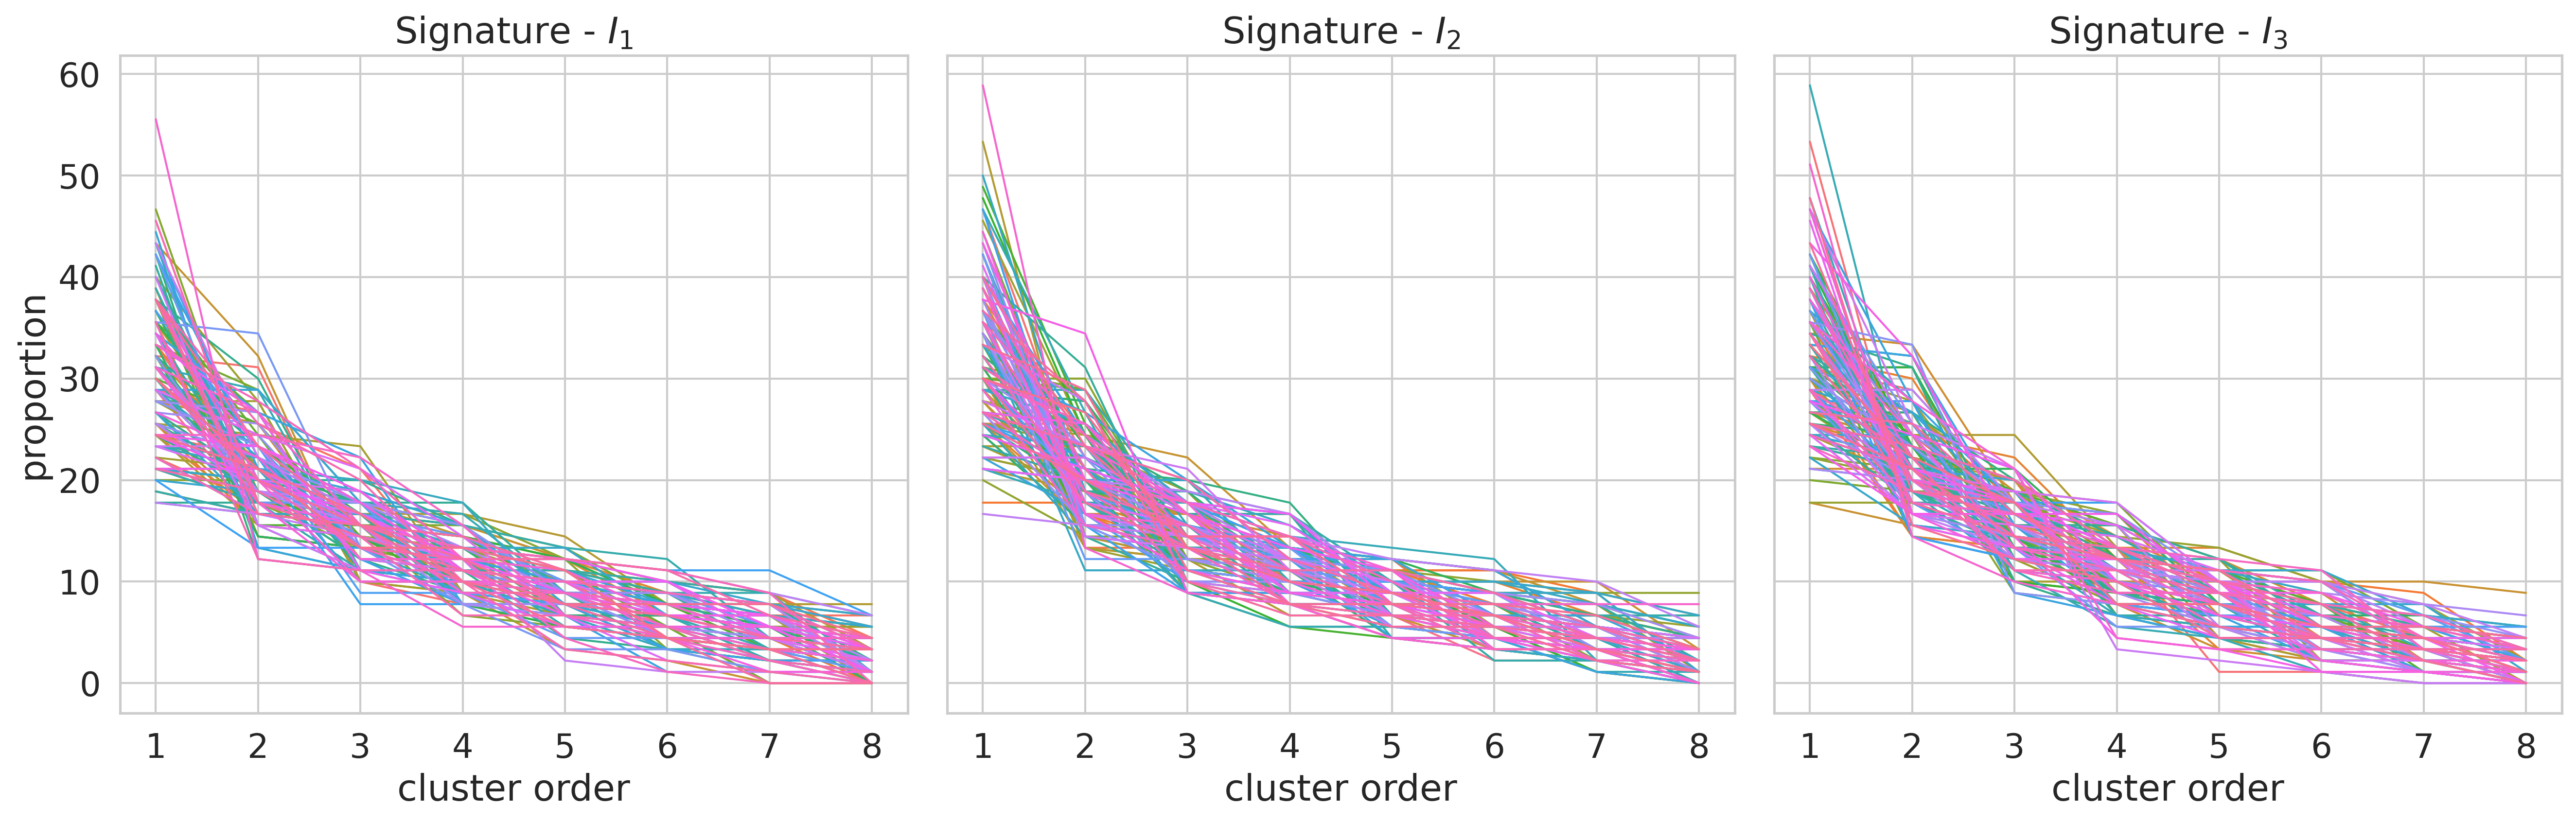
\includegraphics[width=1\linewidth]{figures/tesserae_signature.png}
    \caption{Variations of routine signatures. Each line represents one individual, showing that time allocation across routines remains highly distinctive across segments.}
    \label{fig:signature}
\end{figure}

In S1 (\(N=148\)), we observed strong persistence of routine signatures. Using JSD as distance metric, within-person distances were substantially smaller than between-person distances \dself{0.135}{0.041} vs. \dref{0.164}{0.026} (\dselfdrefpl{226.03}{-8.49}{10^{-3}}), indicating that individuals maintained highly distinctive routine patterns across time. A sanity check using cosine distance produced similar results, with \dself{0.031}{0.021} and \dref{0.055}{0.013} (\dselfdrefpl{246.83}{-11.69}{10^{-3}}).

In S2 (\(N=15\)), the patterns were similar despite the smaller sample size. Routine signatures again showed strong persistence, with JSD distances of \dself{0.222}{0.075} vs. \dref{0.164}{0.026} (\dselfdrefpl{29.99}{-12.13}{10^{-3}}). Robustness check using cosine distances also produced comparable results, with \dself{0.027}{0.026} and \dref{0.096}{0.035} (\dselfdrefp{27.8}{-6.21}{< 10^{-3}}).

In contrast, results from S3 (\(N=125\)) revealed a different finding. Here, individuals exhibited larger within-person distances than in other studies (JSD: \dself{0.253}{0.107}), and these values were not significantly different from the average reference distance \dref{0.248}{0.035} (\dselfdrefp{40.63}{0.28}{0.783}). This indicates that, unlike in S1 and S2, routine signatures in S3 lacked persistence, and individuals could not be reliably distinguished from one another based on their time allocation patterns. Several factors may explain this observation. First, the observation windows in S3 were shorter, with participants contributing on average only 50.6 days of data per segment, compared to the 90-day window in S1 and S2. Second, there were substantial gaps of approximately one year between consecutive 
study waves, which may have introduced major behavioural changes between measurement 
periods. Third, the cohort consisted primarily of college students, a population likely to 
share synchronized schedules (e.g., classes, exams, and campus activities), 
thus reducing inter-individual variability.

\begin{comment}
We further examined routine signatures by ignoring rank order and treating them purely as distributions of time allocation across routines. Under this formulation, the results remained consistent: \dself{0.232}{0.071} and \dref{0.360}{0.059} (\dselfdrefpl{258.42}{-16.86}{10^{-3}}). Notably, the $d_{self}$ values were larger in this case, suggesting that removing rank information reduces within-person similarity.
\end{comment}

\begin{figure}
    \centering
    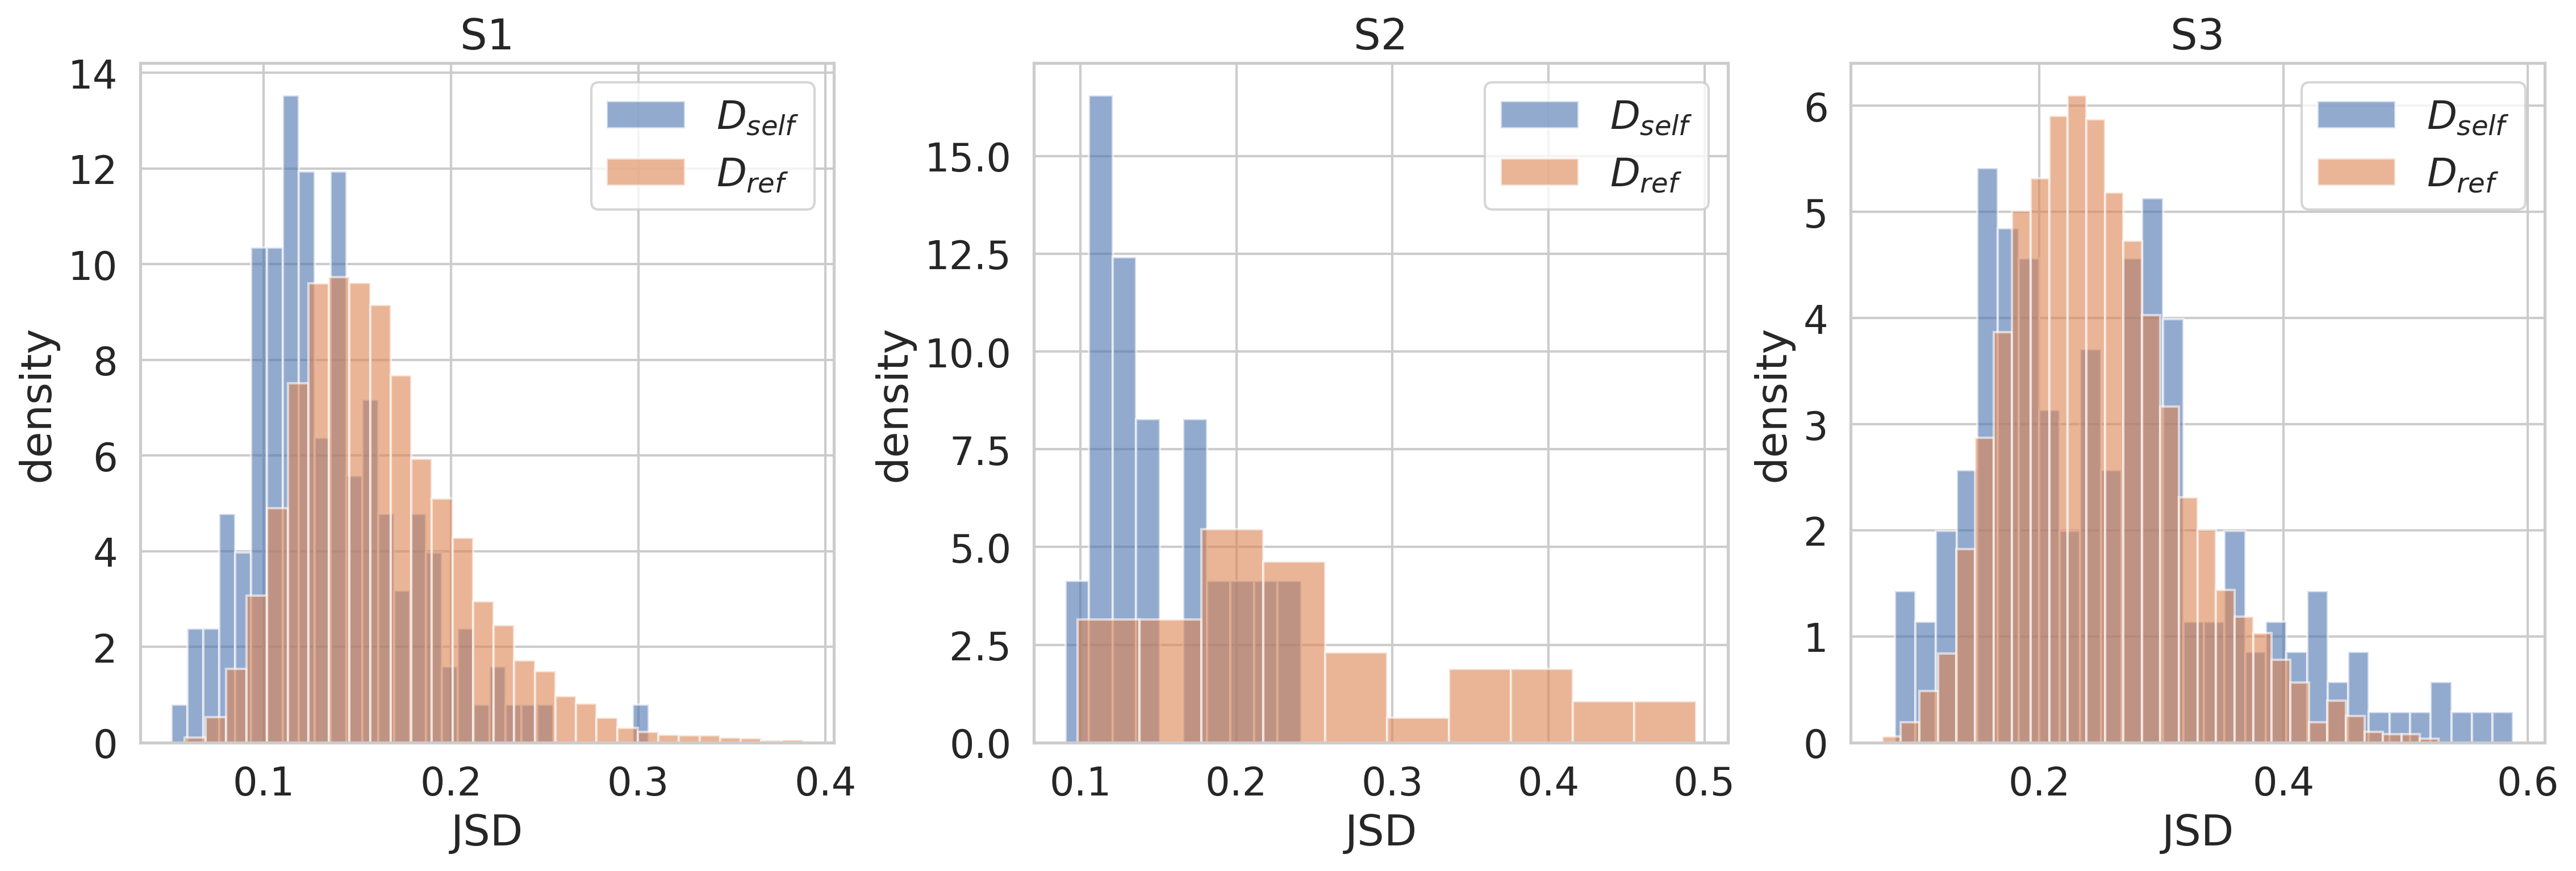
\includegraphics[width=1\linewidth]{figures/combined_dself_dref_ranked_jsd.png}
    \caption{Self-distance and reference-distance}
    \label{fig:dself_dref}
\end{figure}

\subsection*{Transition between routines exhibits similar persistence}

Beyond individual-specific time allocation across routines, we hypothesize that each person’s transition dynamics between routines is also distinctive. That is, people do not follow the same routine every day but instead switch between different latent routine clusters over time in unique ways. For example, one individual may frequently alternate between workday and weekend routines with minimal variability, whereas another may display irregular transitions across several distinct routine types.

To test this hypothesis, we first construct a transition probability matrix 
\(\mathbf{P} \in \mathbb{R}^{K \times K}\) for each participant and segment, 
where \(K\) is the number of routine clusters. We define the transition signature of an individual as the mean row-wise 
distance between their transition matrices across consecutive segments: 
\(d_{\mathrm{self}} = \frac{1}{2} (
D(\mathbf{P}^1, \mathbf{P}^{2}) + D(\mathbf{P}^2, \mathbf{P}^{3}))\). Similarly, the reference distance of individual $i$ was computed by calculating the distance between each participant’s transition matrix with those of all other participants in the same segment, then averaged across 
segments: 
\(d_{\mathrm{ref}} = \frac{1}{3} (
D(\mathbf{P_i}^1, \mathbf{P_j}^{1}) + D(\mathbf{P_i}^2, \mathbf{P_j}^{2}) +
D(\mathbf{P_i}^3, \mathbf{P_j}^{3}))\)

\begin{figure}
    \centering
    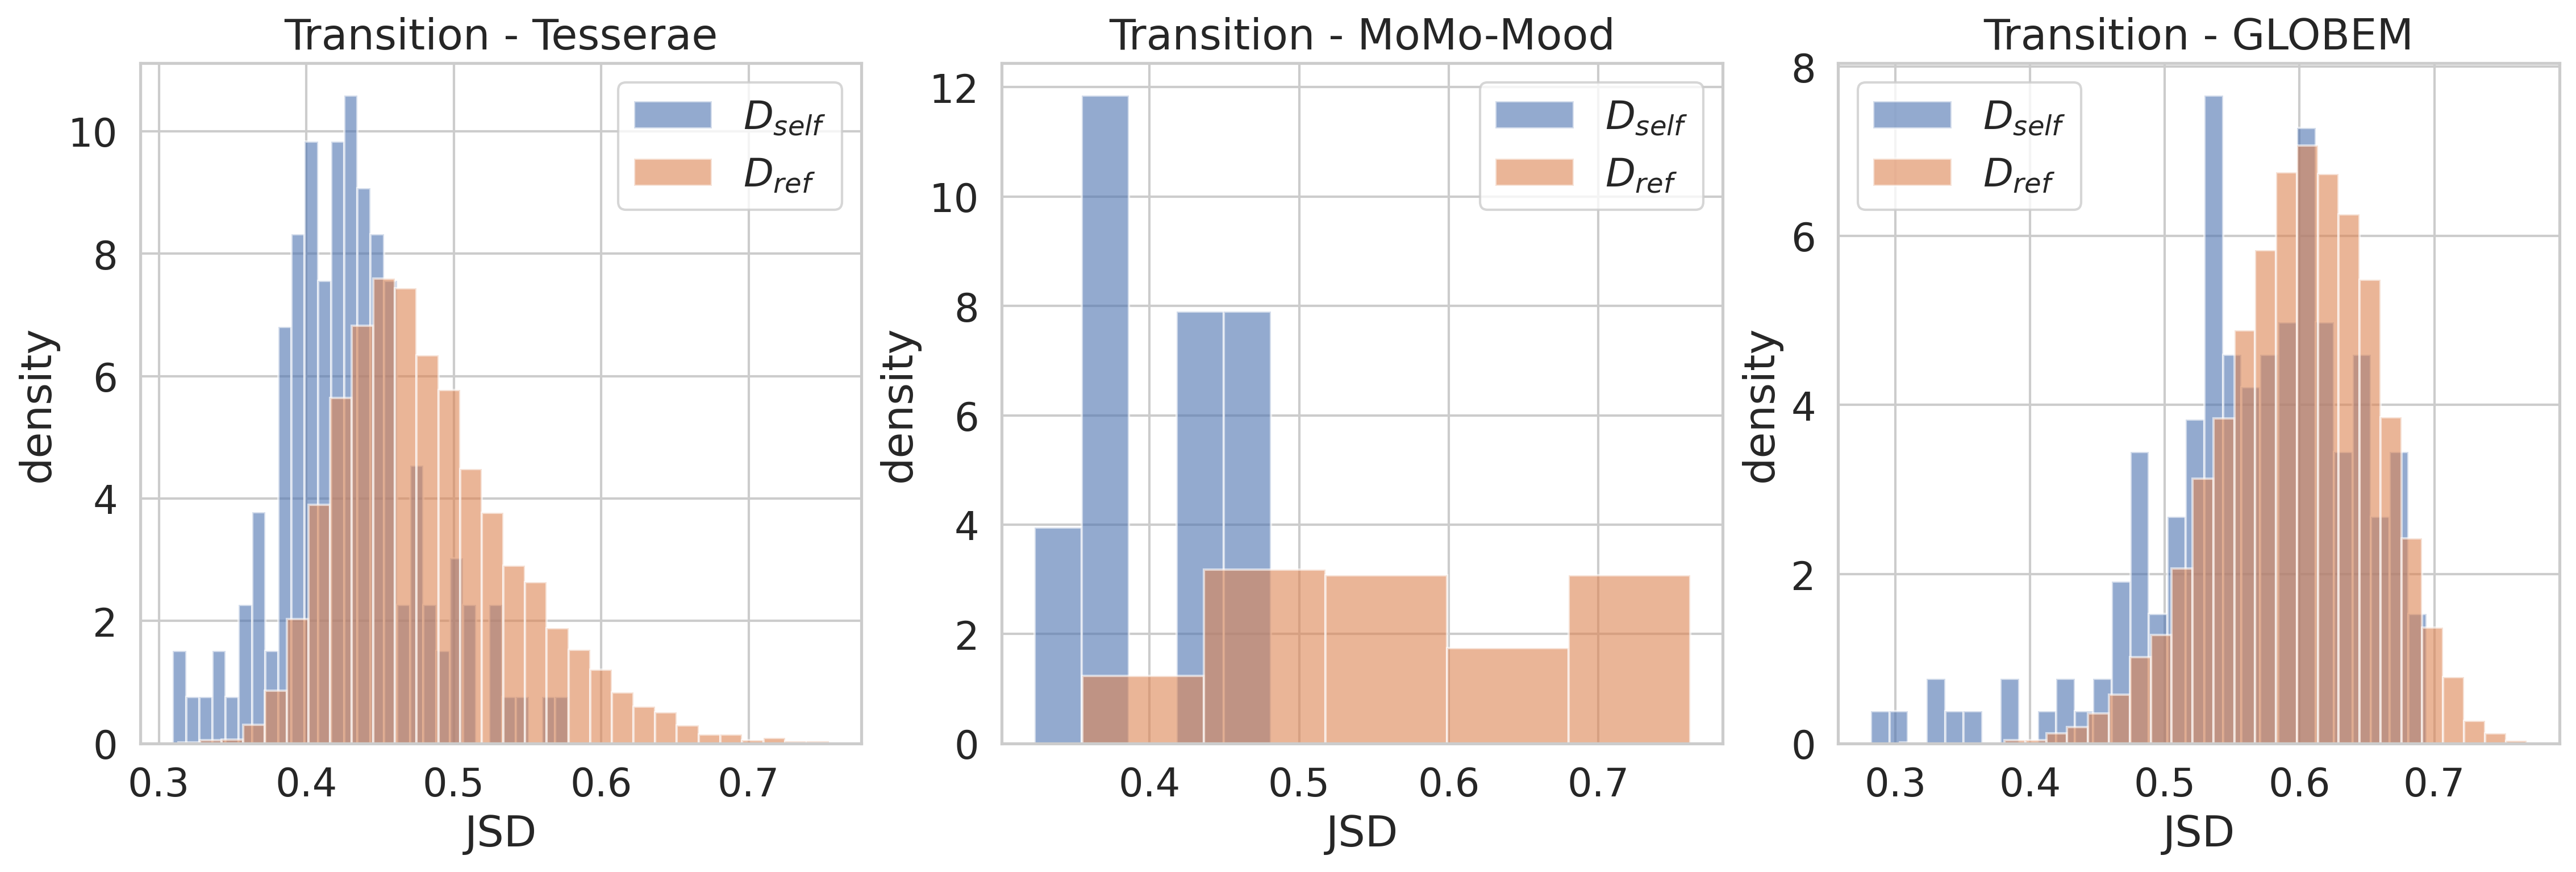
\includegraphics[width=1\linewidth]{figures/combined_transition_dself_dref_jsd.png}
    \caption{Transition signature}
    \label{fig:transition-signature}
\end{figure}

The within-person (\(d_{\text{self}}\)) and between-person (\(d_{\text{ref}}\)) distances of transition matrices for S1 and S2 are shown in \autoref{fig:transition-signature}, generally depicting distribution with similar shape to the self and reference distance of routine signatures. In both studies, individual transition signatures persist accross time segment and were also distiughisable from others. In S1, this distance was \dself{0.481}{0.044}, smaller than the average refrence distance \dref{0.537}{0.029} (\dselfdrefp{255.65}{-12.86}{0.0}). Similarly, in S2, we found \dself{0.458}{0.055} compared to \dref{0.600}{0.046}, \dselfdrefp{28.62}{-7.79}{0.0}.

Note that we did not perform this analysis on S3 due to methodological difference in how cluster of routine was found. In S1 and S2, the whole dataset was used to extract routine 

\subsection*{Factors predicting persistence of routine signature}\label{sec3.3}

Past research has revealed the role of sociodemographic factors \cite{luong2023impact, luong2024sleep, kulshrestha2021web} and personality traits \cite{centellegherPersonalityTraitsEgonetwork2017, alessandrettiUnderstandingInterplaySocial2018, amon2022flexibility} in predicting the persistence of unimodal behavioral routines, such as web browsing, mobility, and physical activity. How do these findings generalize to multimodal behavioral contexts? To investigate this, we built two linear mixed-effects models. The first regressed demographic variables and personality traits on the stability of routine signatures $d_{self}$, while the second modeled their effects on the stability of transition signatures $d_{self\_transition}$. In both models, we included study as a random effect to account for population-specific variability.

% Please add the following required packages to your document preamble:
% \usepackage{booktabs}
% Please add the following required packages to your document preamble:
% \usepackage{booktabs}
\begin{table}[]
\begin{tabular}{@{}lllllll@{}}
\toprule
                  & \multicolumn{3}{c}{d\_self} & \multicolumn{3}{l}{d\_self\_transition} \\ \midrule
                  & beta    & CI    & p-value   & beta        & CI        & p-value       \\
\textbf{Fixed effects}     &         &       &           &             &           &               \\    
Age {[}{]}        &         &       &           &             &           &               \\
Age {[}{]}        &         &       &           &             &           &               \\
Age {[}{]}        &         &       &           &             &           &               \\
Age {[}{]}        &         &       &           &             &           &               \\
Gender            &         &       &           &             &           &               \\
Openness          &         &       &           &             &           &               \\
Conscientiousness &         &       &           &             &           &               \\
Extraversion      &         &       &           &             &           &               \\
Agreeableness     &         &       &           &             &           &               \\
Neuroticism       &         &       &           &             &           &               \\
\textbf{Random effects}    &         &       &           &             &           &               \\
S1                &         &       &           &             &           &               \\
S2                &         &       &           &             &           &               \\
S3                &         &       &           &             &           &               \\ \bottomrule
\end{tabular}
\end{table}

\section*{Discussions}\label{sec4}  

The results in this work exemplified the persistence characteristics of human's routine observed in previous studies, as well as limitations of this persistence. We proposed a framework that models routines as latent behavioural classes and quantifies persistence based on how individuals allocate their time across these classes. Across three independent studies, we found that individuals consistently allocated similar proportions of time to their routines, forming distinctive routine signatures that remained stable over consecutive time segments. However, when examined over longer timescales—such as across years with substantial gaps between observations—this persistence diminished, suggesting that routine signatures are sensitive to large temporal separations and potential life changes.


\subsection*{Limitations}\label{sec4.2}  

Our study has several limitations, both in terms of the data used and proposed method. First, even though we conducted the analysis on a wider range of populations compared to previous studies, the sample size still remains modest. However, given the consistent findings observed in all studies, a wider population would likely yield the same properties. Second, we only account for certain types of routines that occur on a daily basis. Inference of behaviours always come with the obvious risk of missing data, which is very prevalent on certain data type like GPS [cite]. We faced similar problem in this study, with high degree of missing location observed in all studies. Furthermore, routine like communication can be made through various channels, most likely messaging applications nowadays. Communication via traditional like calls and sms in our studies are very sparse or were not captured. We did not have access to application logs in all studies, which prompted us not to include this routine in the analysis. However, given past evidence in the persistence of mobility and communication routines, we can assume that similar characteristics would have been observed should we included those routines in the first place.

\section*{Methods}\label{sec:methods}  

\subsection*{Study description}\label{sec:methods:study_desc}  

We used datasets gathered from three studies, labelled S1, S2, and S3. These datasets were selected based on (1) common use of smartphone-based sensing, (2) the diversity of study populations in terms of geography (Finland and USA), occupation (students and white-collar workers), and mental health status (healthy controls and patients with mental disorder), (3) the diversity the nature of study designs— two continuous monitoring studies and one spanning multiple years. These features aid the generalizability of the findings and .. help test the validity of routine signature. An overview of feature processing and bulding of routine signature is presented in Figure xxx.

\textbf{S1.} The MoMo-Mood study involved patients diagnosed with major depressive episodes, including Major Depressive Disorder (MDD), Bipolar Disorder (BD), and Borderline Personality Disorder (BPD), as well as healthy controls (HC). The study recruited 164 participants from Finland; 133 patients and 31 HCs \cite{aledavood2025multimodal}. Data were collected over a one-year period from smartphones using the AWARE platform \cite{ferreiraAWAREMobileContext2015}, which tracked screen activity, calls and sms, charging behavior, location, accelerometer.

\textbf{S2.} In this study, 757 information workers were recruited across the United States \cite{mattingly2019tesserae}. Participants were provided a Garmin Vivosmart 3 wristband to monitor physical activity, heart rate, sleep, and calories. Additionally, participants installed a custom smartphone app [cite] that passively tracked screen activity, data usage, charging behavior, location, and other phone states.

\textbf{S3.} A multi-year passive sensing datasets of over 700 user-years of data from 497 unique college students \cite{xu2022globem}. Longitudinal data, including location, phone usage, calls, Bluetooth, physical activity, and sleep behavior, were collected from a mobile app and fitness trackers. The study spanned four years, with data collection occurring over 10-week periods each year. 


\subsection*{Features extraction and Preprocessing}\label{sec:methods:features_extraction}  

\textbf{Sleep.} Bed time, wake time, and sleep duration were collected directly from Garmin (Tesserae) and Fitbit (GLOBEM) fitness trackers. In MoMo-Mood, due to the lack of fitness trackers, sleep was estimated using phone lock/unlock status, with the longest lock episode considered sleep. To assess the validity of this proxy, sleep parameters from the same participants were compared to those derived from actigraphy during a two-week validation phase [cite]. The comparison revealed a slight bias but demonstrated adequate correlation between the two methods.

\textbf{Physical activity.} This routine was measured using step count data collected from fitness trackers in the Tesserae and GLOBEM studies. In contrast, for S1, where no fitness trackers were used, mobility was estimated using the standard deviation of the accelerometer magnitude—a method used in prior research [cite]. Accelerometer reading displays a clear 24-hour rhythm with more activity during the day and less so towards the end of the day, justifying the choice of this proxy. To capture daily patterns, activities were aggregated into 4-hour time bins to construct a mobility rhythm, as well as a daily average.

\textbf{Device usage. } The hourly duration of screen use episodes was extracted. Daily rhythms for screen usage were similarly constructed by aggregating their respective durations into 4-hour bins. 

\textbf{Demographics and Personality traits.} All studies collected baseline demographic information at the start. We controlled for age, gender, and occupation, based on the past evidence that these factors influence routine persistence. In addition, personality traits measured using the BFI-10 \cite{rammstedt2007measuring} in S1 and S3, and the NEO-60 \cite{costa1992neo} in S2 were included.

\textbf{Exclusion and normalization}: The records from the first and last day of any user were excluded due to high likelihood of data incompleteness. We excluded participants with fewer than 14 days of data for clustering task. Any day with missing data on device usage, physical activity, or sleep were excluded. Each feature was z-normalized within participants, allowing the model to focus on intra-individual variability. The resulting daily vector contained 13 features (see \autoref{tab:features_list}). Dimensionality reduction was not performed because (1) the feature space is reasonably small and (2) retaining the original variables preserves interpretability of the subsequent clustering results.


\begin{table}[ht]
    \centering
    \begin{tabular}{ll}
        \toprule
        \textbf{Routine} & \textbf{Features} \\
        \midrule
        Physical activity & Step count (S2, S3); accelerometer (S1): daily average + MAEN \\
        Sleep             & bedtime, wake time, sleep duration \\
        Device usage      & Screen usage duration: daily average + MAEN \\
        \bottomrule
    \end{tabular}
    \caption{List of daily behavioral features, grouped by routine domain. MAEN = Morning, Afternoon, Evening, Night segments.}
    \label{tab:features_list}
\end{table}

\subsection*{Building routine cluster using GMM}\label{sec:methods:building_cluster}

All daily feature vectors (of size n features × m days) were modeled using a Gaussian Mixture Model (GMM), where each latent routine is represented by a multivariate Gaussian component. This approach captures both the mean behavioral profile (via the components' mean) and the variability and correlation among features (via the covariance matrices).
Compared to clustering methods like K-Means, GMM offers greater flexibility. First, GMM supports soft clustering, meaning each day is assigned to multiple routine types with varying probabilities, modelling the transition nature of human behavior. Second, each GMM component can be parameterized by the full covariance structure, which captures the interdependencies between routines. For instance, increased phone activity late at night may correlate with delayed bedtime. Third, probabilistic assignments of cluster enable detection of anomalous routines, i.e. days which do not fit into any type of routines.

GMM has two main hyper-parameters: the number of components \(k\) and the covariance type (full, tied, diagonal, or spherical). 
To choose the best model we compared candidates with the Bayesian Information Criterion (BIC). 
For a model using full covariances, we quantified cluster separation by computing all pair-wise Bhattacharyya distances. 
For two multivariate Gaussian clusters \(p_1 \sim \mathcal{N}(\boldsymbol{\mu}_1, \boldsymbol{\Sigma}_1)\) and \(p_2 \sim \mathcal{N}(\boldsymbol{\mu}_2, \boldsymbol{\Sigma}_2)\), the Bhattacharyya distance is

\[
D_B(p_1,p_2)
    = \frac{1}{8}\,
      (\boldsymbol{\mu}_1 - \boldsymbol{\mu}_2)^{\mathsf T}
      \boldsymbol{\Sigma}^{-1}
      (\boldsymbol{\mu}_1 - \boldsymbol{\mu}_2)
      + \frac{1}{2}\,
        \ln\!\left(
          \frac{\det\boldsymbol{\Sigma}}
               {\sqrt{\det\boldsymbol{\Sigma}_1\,\det\boldsymbol{\Sigma}_2}}
        \right),
\]

where
\[
\boldsymbol{\Sigma} = \frac{1}{2} \left( \boldsymbol{\Sigma}_1 + \boldsymbol{\Sigma}_2 \right)
\]
is the average covariance matrix, and \(\boldsymbol{\mu}_1,\boldsymbol{\mu}_2\) are the cluster mean vectors. Larger values indicate better separation and thus more favored models.

We then assigned each day to one of the resulting components. This clustering process was carried out independently for each study. For S3, the dataset spanned multiple academic years, so we fitted the clustering model separately for each year (semester). The tuning process is detailed in Appendix XXX.


\subsection*{Routine signature}\label{sec:methods:signature}  

Social signature describes how individuals persistently distribute their communication efforts across their social contacts. We extend this concept by introducing the notion of a routine signature—the characteristic way in which individuals distribute their time across recurring patterns of daily behavior. This concept aims to capture the persistence in the way people structure their daily lives.

We followed a procedure adapted from prior work on social signatures persistence~\cite{saramaki2014persistence, heydari2018multichannel}. 
For each participant, we first represented every day in terms of behavioral features and assigned GMM. Then, we summarized how often each cluster occurred for that participant by counting the number of days assigned to each cluster. 
To obtain a comparable distribution across individuals, these counts were normalized into proportions, giving the fraction of the participant’s days that belonged to each cluster.  

The clusters were then ranked in descending order of frequency (rank 1 = the most common cluster for that participant). 
The resulting vector of ranked proportions constitutes the \textit{routine signature} of that individual:

\begin{equation}
    \sigma_i = \left(
    \frac{n_{i1}}{\sum_j n_{ij}},\;
    \frac{n_{i2}}{\sum_j n_{ij}},\;
    \ldots,\;
    \frac{n_{ik_i}}{\sum_j n_{ij}}
    \right),
\end{equation}

where \(n_{ij}\) is the number of days participant \(i\) spent in cluster \(j\), and the elements are ordered so that \(\sigma_{i1} \geq \sigma_{i2} \geq \dots\).  

Intuitively, the routine signature reflects the individual pattern of time allocation across latent routines, independent of the cluster labels themselves. In line with the concept of social signatures, we expect this pattern to persist over time.


\begin{figure}[!htbp]
    \centering
    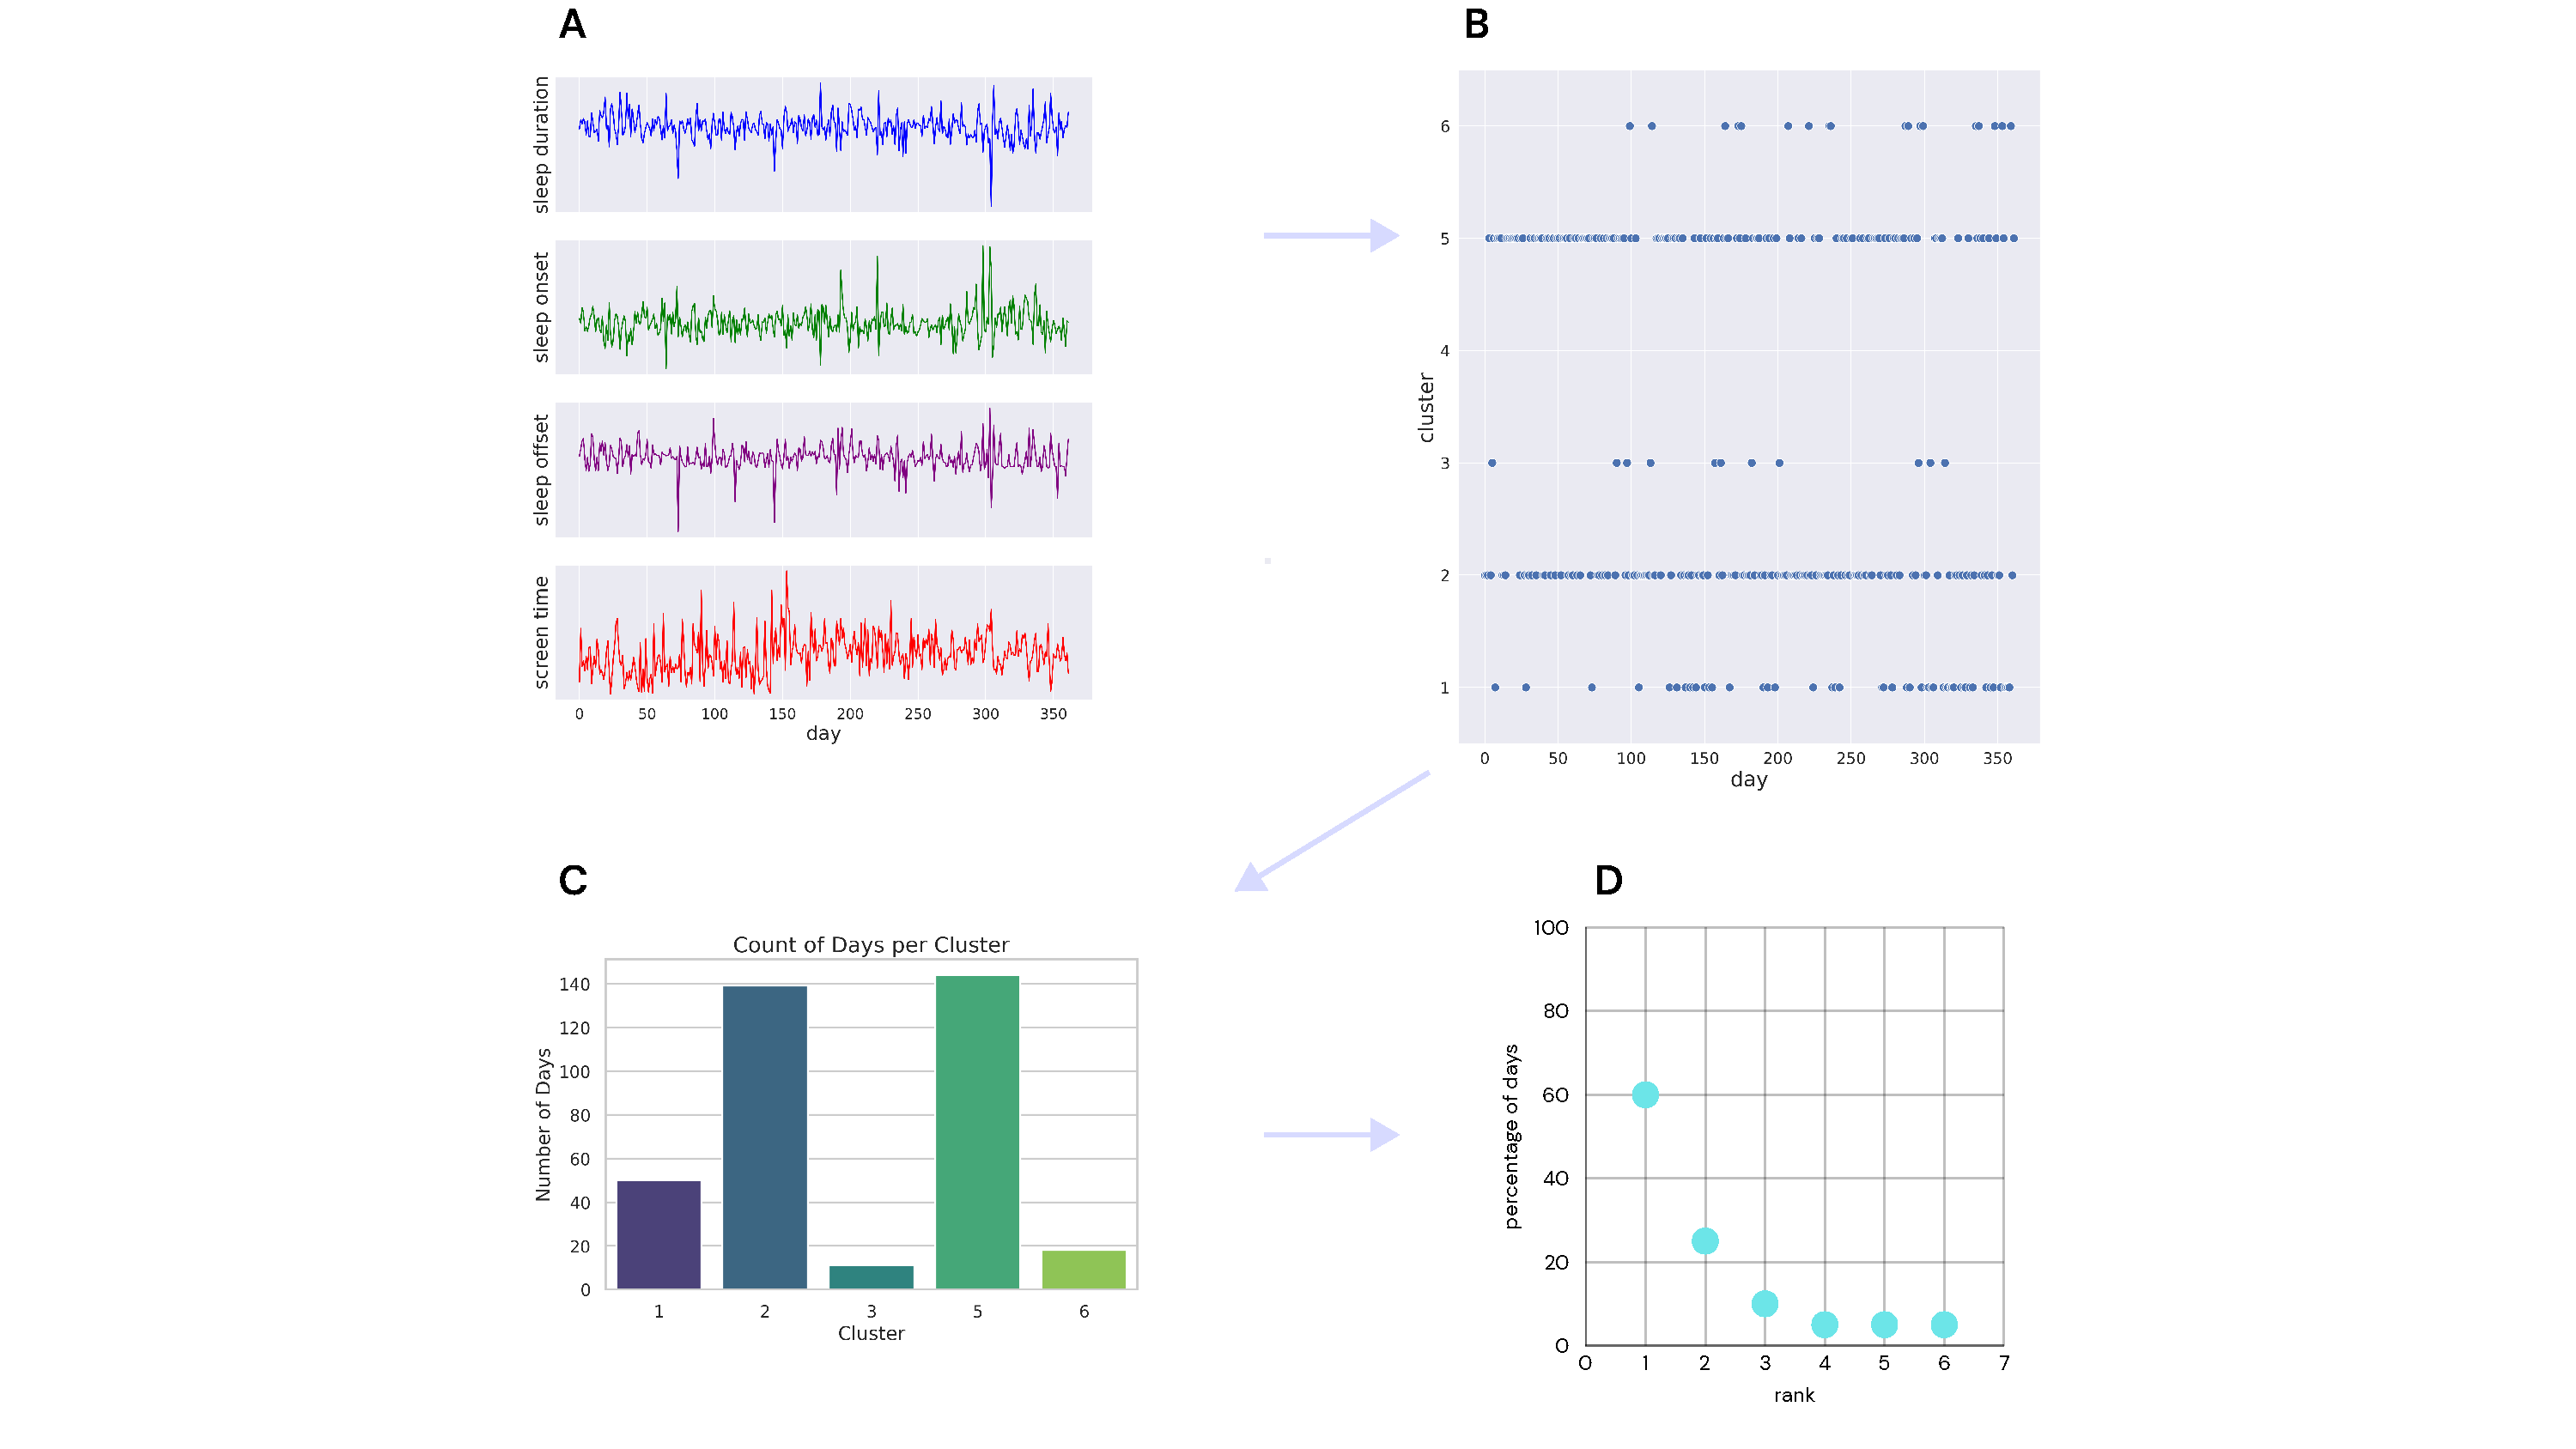
\includegraphics[width=\textwidth]{figures/workflow.pdf}
    \caption{Routine signature workflow. (A) Raw data capturing each person-day’s routine (e.g., sleep times, screen use, activity levels).
(B) a Gaussian Mixture Model (GMM) fitted on the pooled person-day assigns each day to one of the routine clusters.
(C) For each individual, the number of days falling into each GMM‐defined cluster is computed and clusters are ranked by descending day‐counts.
(D) These counts are converted into proportions, giving each person’s “routine signature.}
    \label{fig:routine-sig-workflow}
\end{figure}

\subsection*{Persistence of routine signatures}\label{sec:methods:signature_persistence}  

To quantify the persistence of routine signature, we examine how robust a person maintain the time allocated to their routine over time. For each person, the data was divided into 3 equal time segments. Due to the difference fin study design, the segmenting strategy was done differently for each dataset. For S1 and S2, each segment consisted of 90 days of data, hence we retained users with at least 270 data days. For S3, each segment equals to each wave, i.e 10 weeks of data and we retain the users that participated in at least 2 waves of the study. We defined persistence of routine as the distance between the routine signatures in 3 time segments, using the Jensen-Shannon divergence (JSD) \cite{lin1991divergence}:

\begin{equation}
JSD(\sigma_1, \sigma_2) = H(\frac{\sigma_1 + \sigma_2}{2}) - \frac{1}{2}[H(\sigma_1) + H(\sigma_2)]
\end{equation}

where $\sigma_1$ and $\sigma_1$ are the social signatures defined in Eq. 1, and $H(\sigma)$ is the Shannon entropy of $\sigma$.

To determine how well one maintains their routines over time, we define $d_{self} = 0.5 * (d_{12} + d_{23})$. We validate individual's persistence against the population, by computing the reference distance $d_{ref} = \frac{1}{3}* (d_{i1j1} + d_{i2j2}  + d_{i3j3} )$. That is, we compute the routine signature in each time split of individual $i$ against that from the same time split of individual $j$.


% Uncomment to include appendix
%% Preamble additions (recommended)
% \usepackage{graphicx}
% \usepackage{subcaption}
% \usepackage{placeins}   % for \FloatBarrier
% \usepackage{float}      % if you want [H] placement (optional)

\section{Appendices}

\begin{appendices}

% ---------- A: GMM model tuning ----------
\clearpage                    % start this appendix section on a new page
\section{GMM model tuning}

Model tuning across all cohorts favored Gaussian mixtures with full covariance matrices, yielding lower Bayesian Information Criterion (BIC; lower is better) and higher average Bhattacharyya distances between components (greater separation). Performance improved up to \(K=8\) and then showed diminishing returns, so we fixed \(K=8\) for the main analyses. All principal findings were confirmed in a sensitivity analysis with \(K \in \{6,\ldots,11\}\).


\begin{figure}[p]
  \centering
  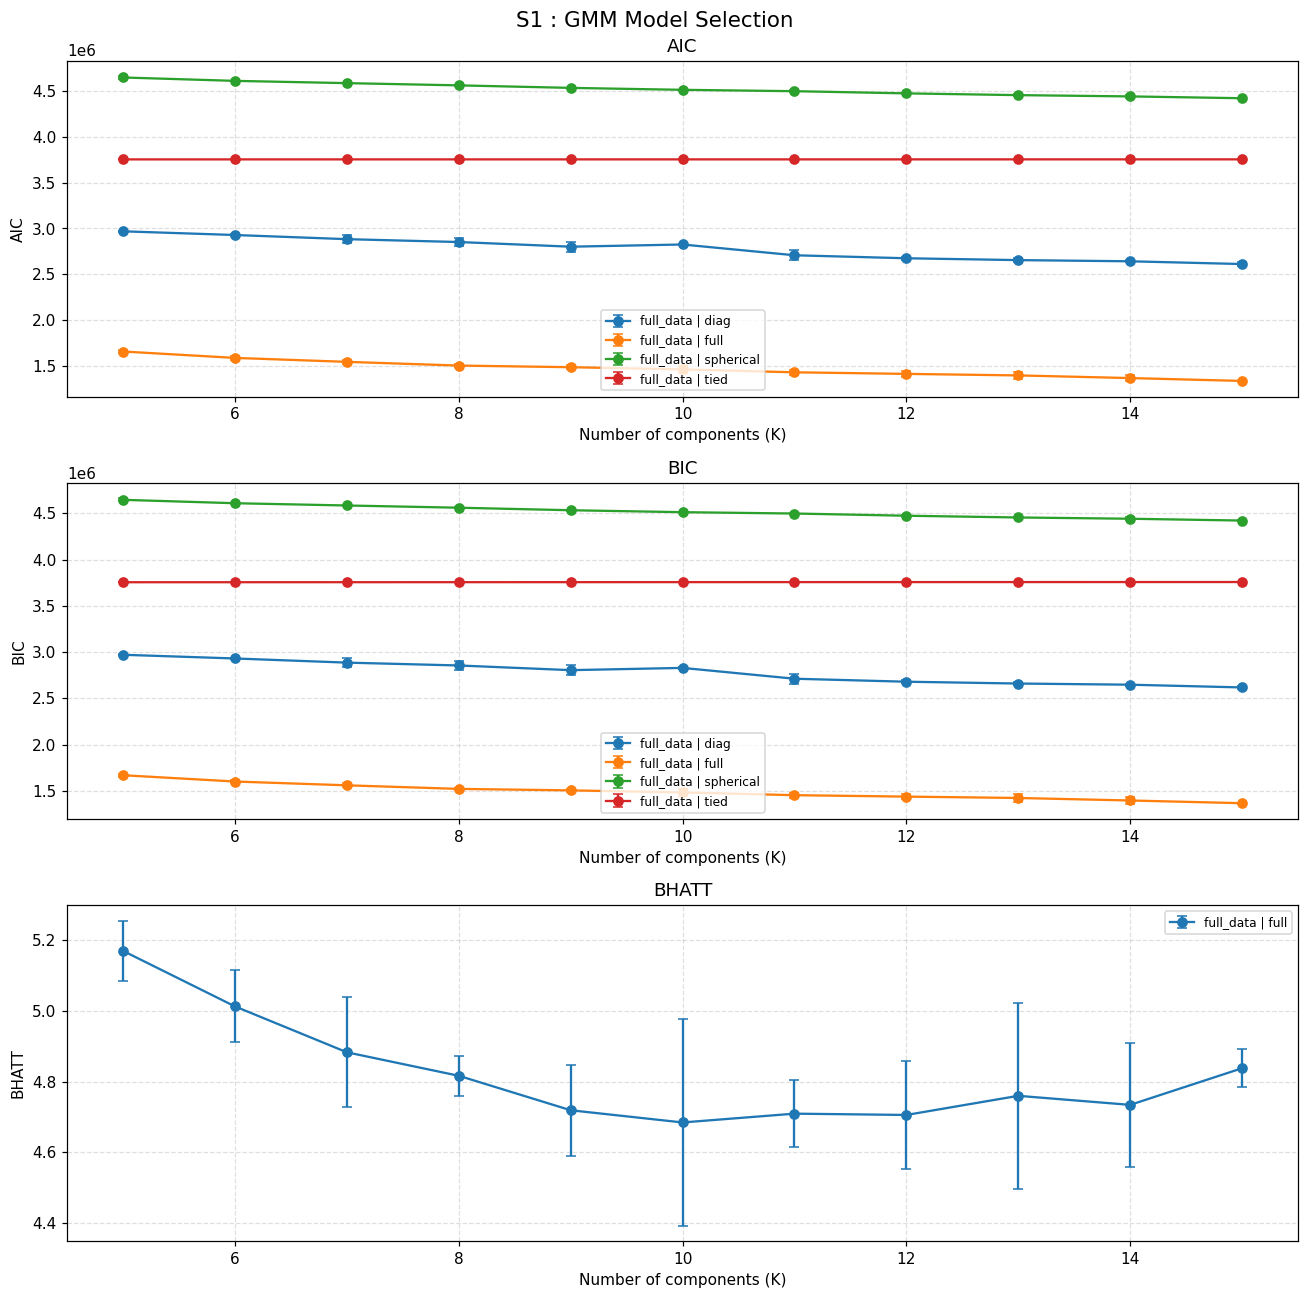
\includegraphics[width=\linewidth]{figures/appendix/tesserae_gmm_model_selection.png}
  \caption{Tesserae: Model selection}
  \label{fig:tesserae_model_selection}
\end{figure}

\begin{figure}[p]
  \centering
  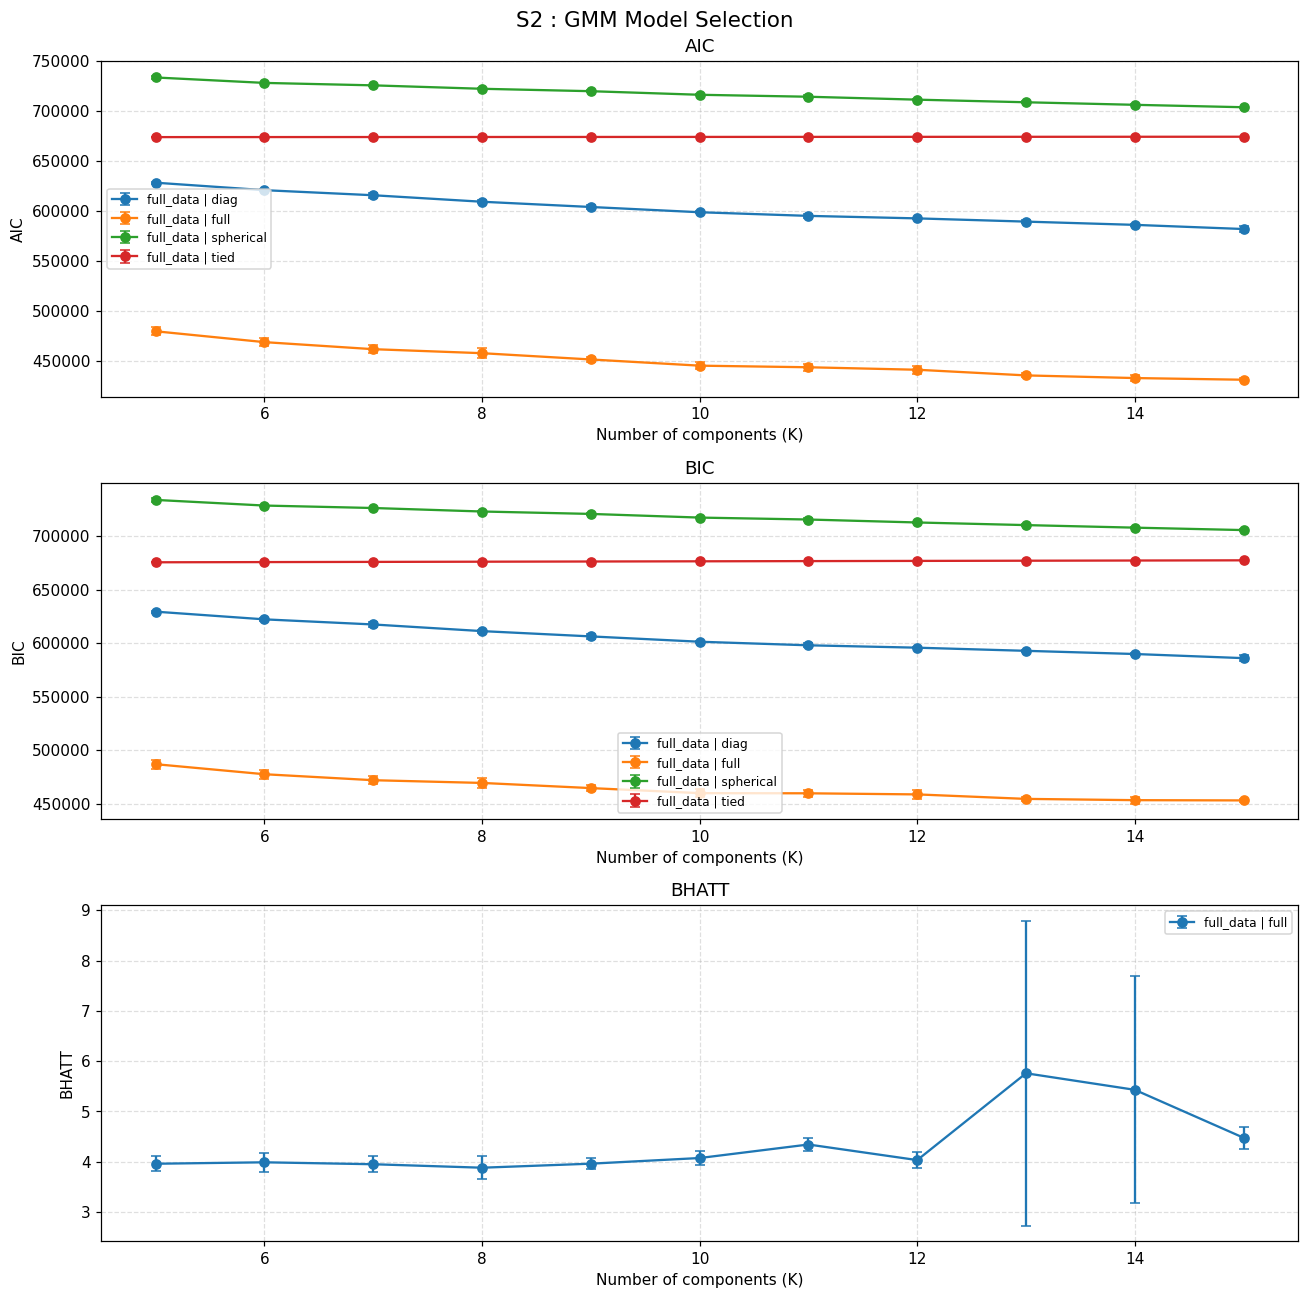
\includegraphics[width=\linewidth]{figures/appendix/momo_gmm_model_selection.png}
  \caption{MoMo-Mood: Model selection}
  \label{fig:momo_gmm_model_selection}
\end{figure}

\begin{figure}[p]
  \centering
  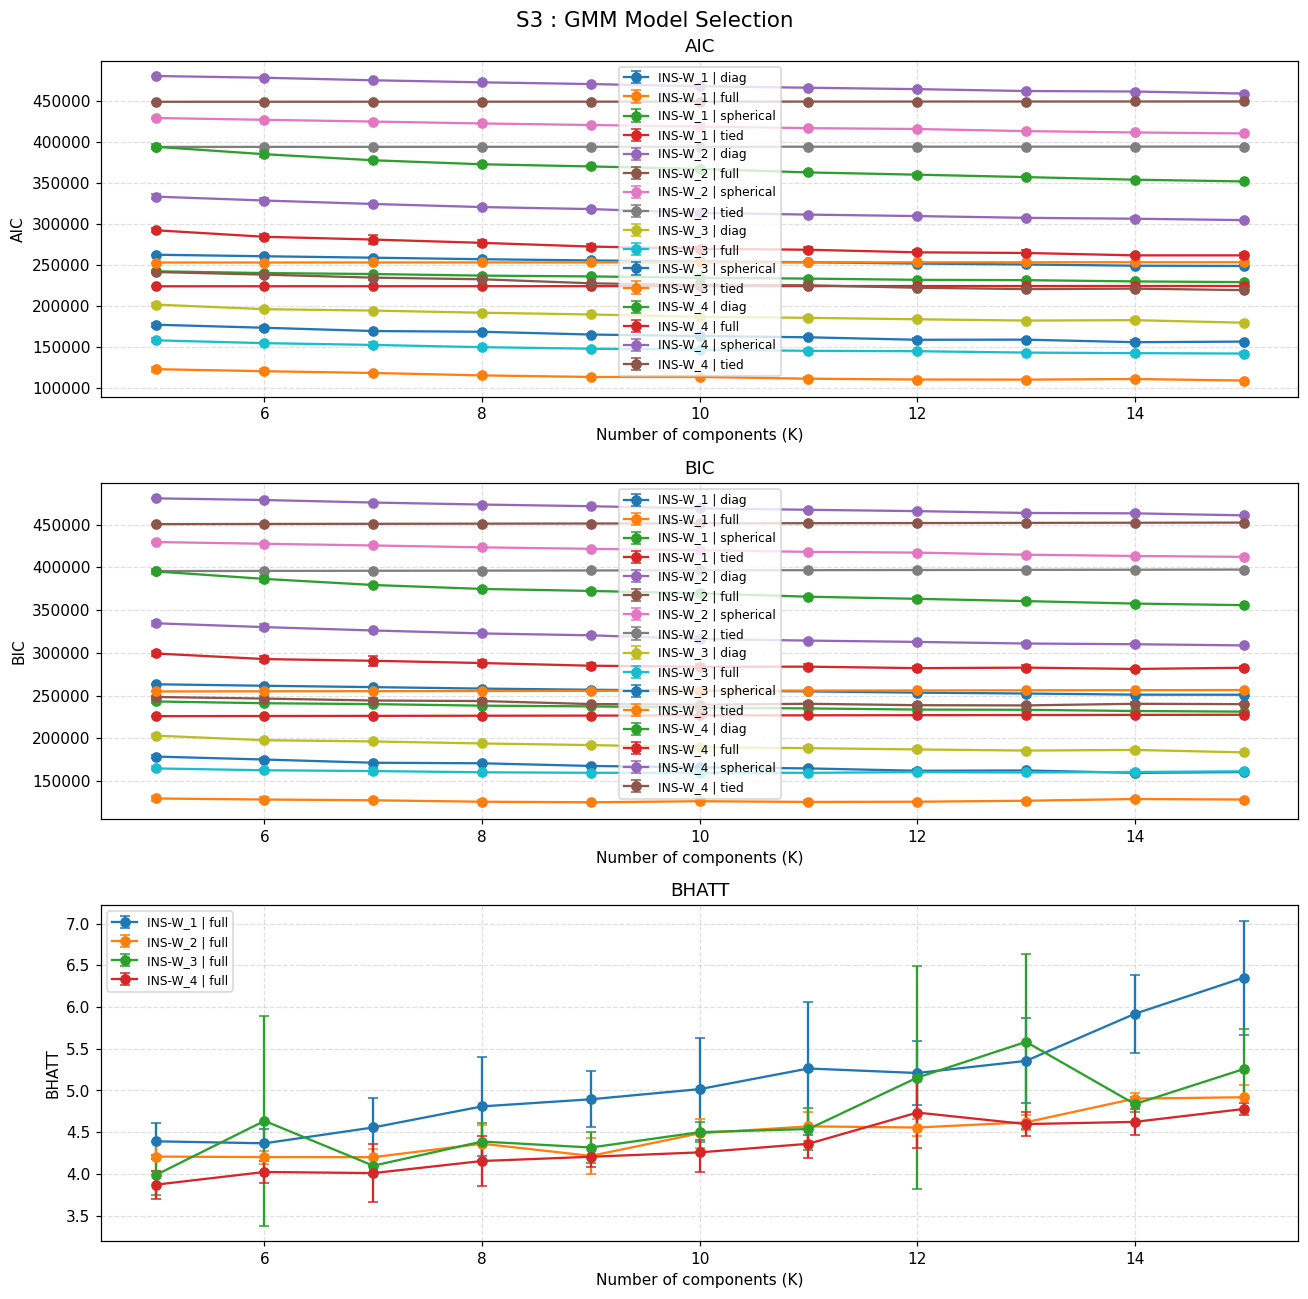
\includegraphics[width=\linewidth]{figures/appendix/globem_gmm_model_selection.png}
  \caption{GLOBEM: Model selection}
  \label{fig:globem_gmm_model_selection}
\end{figure}

\FloatBarrier                 % ensure these floats don’t spill into the next section

% ---------- B: Cluster properties ----------
\clearpage
\section{Cluster properties of MoMo-Mood and GLOBEM}

\autoref{fig:momo_centroid_summary} and \autoref{fig:globem_centroids} describe the cluster characteristics of the MoMo-Mood and GLOBEM studies, respectively. Across both datasets, a few dominant clusters account for the majority of time, while other clusters reflect free day routines, for example, elevated nightly activity or increased nighttime screen use.

\begin{figure}[p]
  \centering
  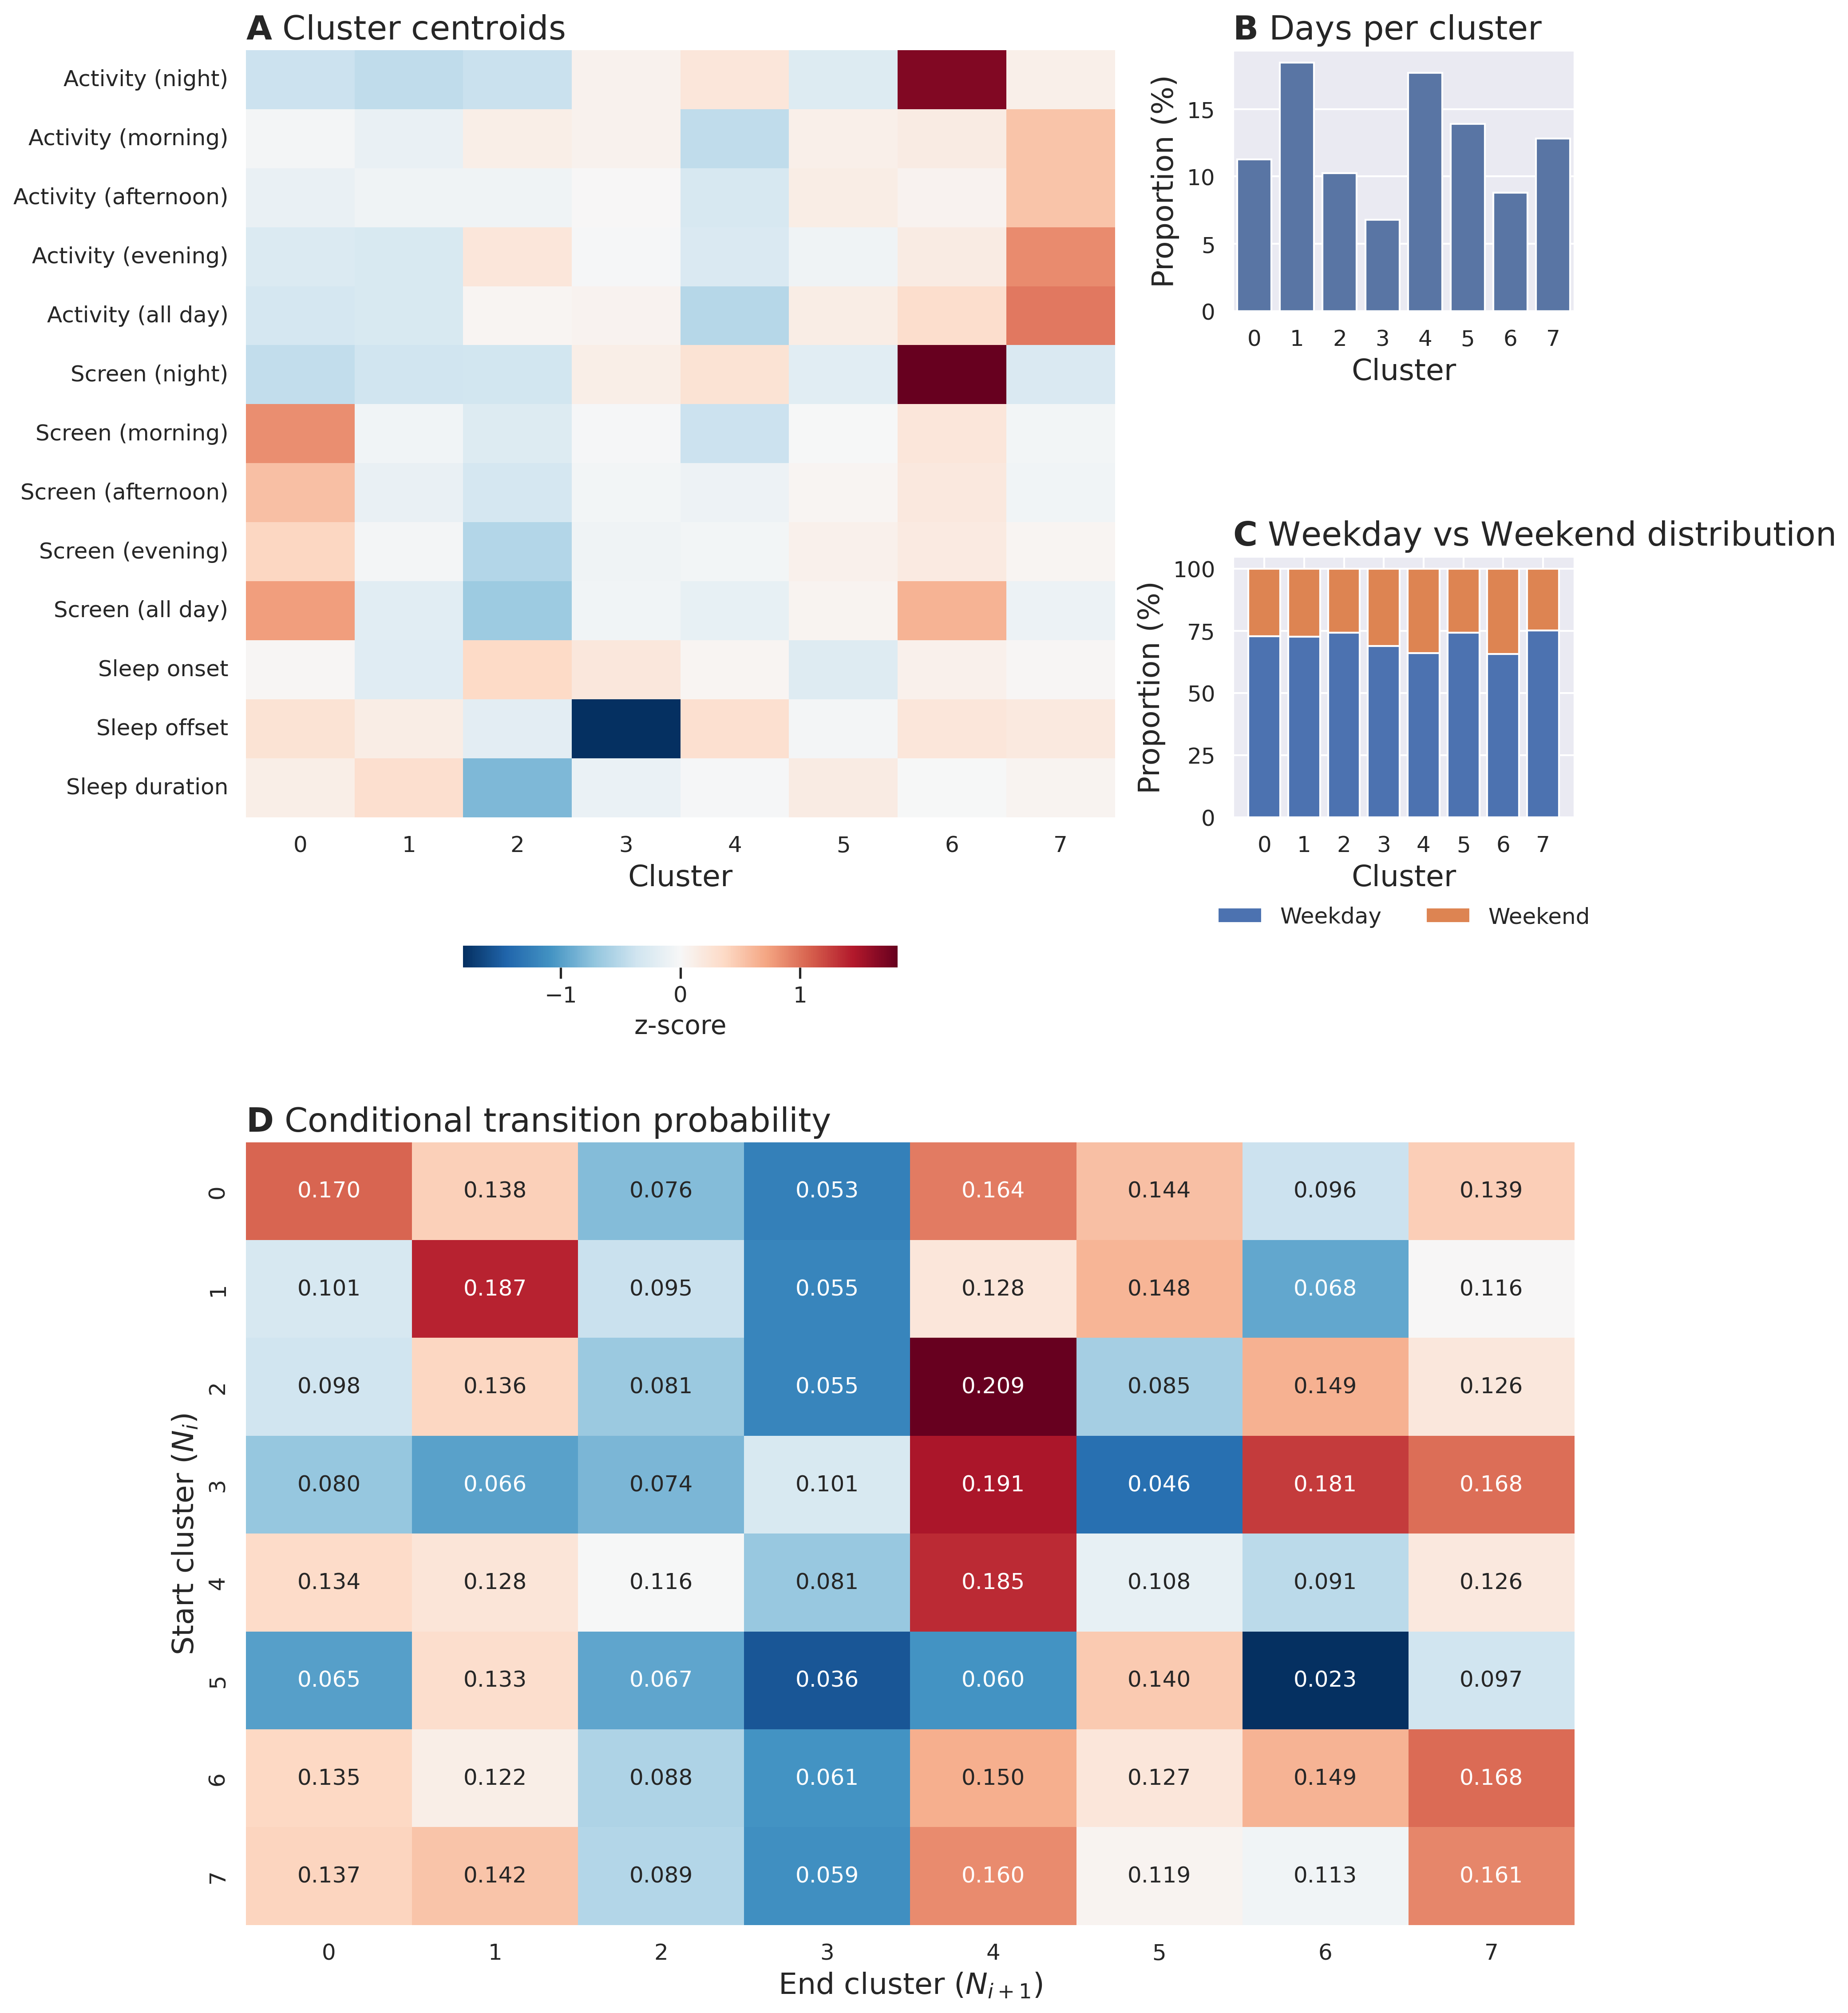
\includegraphics[width=\linewidth]{figures/appendix/momo_summary.png}
  \caption{MoMo-Mood: Cluster centroid characteristics}
  \label{fig:momo_centroid_summary}
\end{figure}

% 2x2 subfigures for GLOBEM centroid characteristics (example filenames 1–4)
\begin{figure}[p]
  \centering

  \begin{subfigure}[t]{0.485\textwidth}
    \centering
    \includegraphics[width=\linewidth]{figures/appendix/globem_INS-W_1_summary.png}
    \caption{Cluster 1}
    \label{fig:globem_centroids_a}
  \end{subfigure}\hfill
  \begin{subfigure}[t]{0.485\textwidth}
    \centering
    \includegraphics[width=\linewidth]{figures/appendix/globem_INS-W_2_summary.png}
    \caption{Cluster 2}
    \label{fig:globem_centroids_b}
  \end{subfigure}

  \medskip

  \begin{subfigure}[t]{0.485\textwidth}
    \centering
    \includegraphics[width=\linewidth]{figures/appendix/globem_INS-W_3_summary.png}
    \caption{Cluster 3}
    \label{fig:globem_centroids_c}
  \end{subfigure}\hfill
  \begin{subfigure}[t]{0.485\textwidth}
    \centering
    \includegraphics[width=\linewidth]{figures/appendix/globem_INS-W_4_summary.png}
    \caption{Cluster 4}
    \label{fig:globem_centroids_d}
  \end{subfigure}

  \caption{GLOBEM: Cluster centroid characteristics.}
  \label{fig:globem_centroids}
\end{figure}


% ---------- C: Signature with varying K ----------
\clearpage
\section{Signature with varying K components}

% (Add your figures/tables for this section here; using [p] + \FloatBarrier keeps them on this section’s pages.)

% \begin{figure}[p]
%   \centering
%   \includegraphics[width=\linewidth]{figures/appendix/signature_varying_K.png}
%   \caption{Signature stability under varying number of components K.}
%   \label{fig:signature_varying_K}
% \end{figure}
% \FloatBarrier

\end{appendices}


%%===========================================================================================%%
%% If you are submitting to one of the Nature Portfolio journals, using the eJP submission   %%
%% system, please include the references within the manuscript file itself. You may do this  %%
%% by copying the reference list from your .bbl file, paste it into the main manuscript .tex %%
%% file, and delete the associated \verb+\bibliography+ commands.                            %%
%%===========================================================================================%%

\bibliography{sn-bibliography}% common bib file
%% if required, the content of .bbl file can be included here once bbl is generated
%%\input sn-article.bbl


\end{document}
